\documentclass[a4paper, 12pt, twoside]{report} % Formato de plantilla
\raggedbottom % Para que el formato twoside no haga vfill si hay cosas que no ocupan una cara entera
\usepackage{tex/estilo}

% Comienzo del documento
\begin{document}
	%-----------------------------------------------------------------------------------
	% Portada 
	% Portada
\begin{titlepage}
\newpage
\changepage{2in}{}{}{-0.2in}{}{-0.6in}{}{}{}
\thispagestyle{empty}
\newpagecolor{orange}\afterpage{\restorepagecolor}
	
	\begin{center}

	\renewcommand{\baselinestretch}{2.0}
\textbf{\Large UNIVERSIDAD POLIT\'{E}CNICA DE MADRID}\\
\textbf{\large ESCUELA T\'{E}CNICA SUPERIOR \\ DE INGENIEROS DE TELECOMUNICACI\'{O}N}\\
	\vspace{1.0cm}
	\includegraphics[width=8cm]{\logoportadaU}
	\vspace{0.5cm} \\

\textbf{\Large \grado}\\
	\vspace{0.5cm}

\textbf{TRABAJO FIN DE GRADO}\\
	\vspace{3.5cm}
	\baselineskip=20pt

\textbf{\textbf{\Large \titulo}}\\
	\vspace{6.5cm}
	\baselineskip = 20pt

\textbf{\Large \autor} \\
	\vspace{1cm}

		\textbf{\Large \fecha} \\

	\end{center}

\afterpage{\blankpage}

\end{titlepage}

	%%%%%%%%%%%%%%%%%%%%%% PORTADA CON TUTOR %%%%%%%%%%%%%%%%%%
\newpage
\changepage{2in}{}{}{-0.2in}{}{-0.6in}{}{}{}

	\thispagestyle{empty}
	\begin{center}

	\renewcommand{\baselinestretch}{2.0}

\textbf{\Large UNIVERSIDAD POLIT\'{E}CNICA DE MADRID}\\
\textbf{\large ESCUELA T\'{E}CNICA SUPERIOR \\DE INGENIEROS DE TELECOMUNICACI\'{O}N}\\

	\vspace{1.0cm}
	\includegraphics[width=8cm]{\logoportadaD}
	\vspace{0.5cm}

	\textbf{\Large \grado}\\
	\vspace{0.5cm}
	\textbf{TRABAJO FIN DE GRADO}\\

	\vspace{3.5cm}

        \baselineskip=20pt
        \textbf{\textbf{\Large \titulo}}\\

        \vspace{4.5cm}
        \baselineskip = 20pt


        \textbf{\Large Autor} \\
        \textbf{\Large \autor} \\

  \vspace{1cm}

  \baselineskip = 20pt
        
	\textbf{\Large Tutor} \\
  	\textbf{\Large \tutor} \\

  \vspace{1cm}
        \textbf{\Large \fecha} \\

	\end{center}

\afterpage{\blankpage}

	%-----------------------------------------------------------------------------------
	% Agradecimientos
    \input{tex/c0-3_agradecimientos}
    % Abstract 
	% Abstract 
\newpage
\thispagestyle{empty}
\addcontentsline{toc}{chapter}{Abstract}
\section*{Abstract}
Ejemplo abstract
\afterpage{\blankpage}


	% Resumen
	\input{tex/c0-5_resumen}
    % Glosario 
	\input{tex/c0-6_glosario}
	% ----------------------------------------------------------------------------------
	% TOC
	\tableofcontents
	% Figuras
	\listoffigures
	\afterpage{\blankpage}
	\addcontentsline{toc}{chapter}{\listfigurename}
    % Tablas
    \listoftables
    \afterpage{\blankpage}
    \addcontentsline{toc}{chapter}{\listtablename}
	%-----------------------------------------------------------------------------------
	% Contenido
	% Introducción
\newpage
\setcounter{page}{1}
\pagenumbering{arabic}
\chapter{Introducción}  
  En este capítulo se va a presentar el proyecto a fin de dar una primera impresión así como proporcionar una idea de lo que se va a ir detallando en capítulos posteriores.

\section{Motivación} \label{sec:mot}
  La creciente importancia que la digitalización ha alcanzado en el ámbito empresarial ha impactado directamente en las necesidades de ciberseguridad de las organizaciones. Buena parte de los ciudadanos, la mayoría de las empresas y casi la totalidad de los gobiernos son víctimas, a diario, de millones de ciberataques con un grado variable de sofisticación e impacto y, lo que es más preocupante, en su mayoría imperceptibles. La sustracción de información sensible o de datos de carácter personal, los ciberdelitos de naturaleza económica y la inutilización de sistemas militares, industriales, empresariales e incluso de infraestructuras críticas, son los principales objetivos de la gran mayoría de los ciberataques que acontecen hoy en día.

  En este contexto, existe una creciente demanda de profesionales en el ámbito de la ciberseguridad por parte de gobiernos y empresas. La capacitación continua de estos profesionales es esencial para disponer de una ciberdefensa que permita establecer las medidas de seguridad apropiadas de los ciberespacios que protegen. Esta capacitación  requiere de un nivel de innovación continuo únicamente proporcionado por entornos como los Cyber Range.

  Un Cyber Range es una plataforma virtual que permite simular entornos operativos reales para la formación y el entrenamiento (individual o colectivo) de profesionales así como la experimentación,  el testeo y  la validación de nuevos conceptos, tecnologías, técnicas y tácticas de ciberseguridad y ciberdefensa.

  Con el fin de hacer los Cyber Range lo más eficaces posible surge este trabajo de fin de grado. Se entiende por eficaz un Cyber Range que cumple los siguientes requisitos:
  \begin{itemize}
    \item Escenarios accesibles en tiempo y forma por los profesionales autorizados para su utilización de una forma muy sencilla.
    \item Escalabilidad y flexibilidad para poder responder a las necesidades de los responsables en materia de ciberseguridad y ciberdefensa en función de la naturaleza de las actividades que lleven a cabo.
    \item Entorno seguro que permita a los usuarios ejecutar las actividades sin poner en riesgo los sistemas en producción e información clasificada o sensible.
  \end{itemize}

  Estos aspectos contribuyen a una mejor formación y entreno de los profesionales de seguridad, a la par que facilitan el cumplimiento de las estrategias de ciberseguridad.

\section{Objetivos} \label{sec:obj}
  El objetivo de este trabajo es realizar despliegues de red heterogéneos virtualizados, aplicables a plataformas Cyber Range para la formación y entrenamiento en el campo de la ciberseguridad. El trabajo se centra principalmente en el despliegue de la infraestructura así como su interconexión, y no en la configuración a fondo de todos los elementos para la realización de tests de intrusión específicos.

  Para alcanzar el objetivo final, se han identificado una serie de subobjetivos, desde lo más básico hasta lo más complejo, que en conjunto permitirán obtener el resultado deseado:

  \begin{table}[h]
    \begin{center}
      \begin{tabular}{ | w{c}{1cm} | m{14cm} | }
        \hline\rowcolor{oranget} \textbf{Id} & \textbf{Objetivo del TFG} \\ \hline
        O1 & Determinar los escenarios a desplegar, intentando que estos reflejen situaciones lo más realistas posible. \\ \hline\rowcolor{oranger}
        O2 & Posibilitar un despliegue de infraestructura que sea modelable mediante variables, escalable, portable y seguro. \\ \hline
        O3 & Diseñar y configurar la comunicación entre los elementos que componen los escenarios. \\ \hline\rowcolor{oranger}
        O4 & Pese a no ser el objetivo principal del trabajo, desarrollar una herramienta que sirva como base para la configuración software de dichos escenarios. \\ \hline
      \end{tabular}
      \caption{Objetivos planteados}
      \label{tab:objs}
    \end{center}
  \end{table}

\section{Estructura del documento} \label{sec:est}
  El presente documento se secciona en capítulos. A fin de tener una visión global de las distintas fases, se muestra a continuación cada uno de ellos junto a una breve descripción:

  \textbf{Capítulo 1.} Es la introducción al TFG, donde se proporciona una visión global y se describe la motivación de este así como los objetivos a conseguir.

  \textbf{Capítulo 2.} Presenta el estado del arte, resumiendo las tecnologías empleadas en el proyecto y su comparación con opciones alternativas.

  \textbf{Capítulo 3.} Diseño de la solución a implementar, basada en los requisitos identificados. Presentación de las  diferentes etapas a seguir para ello.

  \textbf{Capítulo 4.} Se desarrolla la lógica seguida para implementar cada uno de los escenarios.

  \textbf{Capítulo 5.} Resumen de los resultados obtenidos tras la fase de desarrollo reforzado con tests que lo prueban.

  \textbf{Capítulo 6.} Conclusiones y problemas surgidos a raíz de la realización del proyecto. Líneas futuras sobre las que trabajar.

	% Estado del arte
\chapter{Estado del arte}
\section{Tecnologías de virtualización}
Se podría decir que la virtualización es ya uno de los pilares fundamentales del mundo IT debido a las grandes ventajas que proporciona. Previo al desarrollo de las tecnologías y tipos de virtualización disponibles, es conveniente explicar en qué consiste la virtualización, que no es más que una representación mediante software de un entorno físico o recurso tecnológico, como pueden ser aplicaciones, servidores o almacenamiento. 

Gracias a esta tecnología, es posible contar con varios ordenadores virtuales en el mismo hardware, donde cada uno de ellos puede interactuar de forma independiente y ejecutar sistemas operativos o aplicaciones diferentes mientras comparten los recursos de una sola máquina host. Al crear varios recursos a partir de un único equipo o servidor, la virtualización mejora la escalabilidad y las cargas de trabajo, al tiempo que permite usar menos servidores y reducir el consumo de energía, los costos de infraestructura y el mantenimiento.

En función del sistema a simular, podemos encontrar diferentes categorías, un ejemplo es la virtualización de red, que consiste en crear redes virtuales sobre redes físicas o reproducir completamente redes físicas en software. Otro ejemplo sería la virtualización de almacenamiento, que combina varios dispositivos de almacenamiento en red, con la apariencia de una única unidad o dispositivo de almacenamiento, accesible por varios usuarios. Podríamos enumerar más tipos de virtualización, pero en lo que a este trabajo respecta vamos a centrarnos en la virtualización de software, que separa las aplicaciones del hardware y el sistema operativo, y en la que distinguimos dos subtipos: virtualización mediante hipervisor y virtualización en contenedores.

\subsection{Virtualización mediante hipervisor}
Una máquina virtual es un software que ejecuta programas o procesos como si fuera la máquina física. Es decir, se abstrae el hardware y se representa con una capa de software que proporciona una interfaz igual que el hardware, de forma que sobre ella podemos instalar uno o varios sistema operativos invitados o guests distintos. Esta capa de software también se encarga de repartir y aislar los recursos del host entre las VM, de manera que el host queda protegido si falla una VM, y las VM estén protegidas entre ellas. Pues bien, cuando hablamos de esta capa de software estamos hablando de lo que se conoce como hipervisor. 

Como ya se ha mencionado, un hipervisor es una capa intermedia de software que permite al ordenador anfitrión prestar soporte a varias máquinas virtuales mediante el uso compartido de sus recursos. Cuando se ejecuta una instrucción en el SO invitado, el hipervisor la coje y la ejecuta en el SO anfitrión. En este proceso, el SO no diferencia entre ejecutar procesos en la máquina virtual o en la física, lo que representa plenamente el concepto de virtualización.

Dentro de los hipervisores, podemos distinguir dos tipos. El primero es el Tipo 1, conocido también como hipervisor nativo o bare-metal. Este hipervisor se ejecuta directamente sobre el hardware en lugar de un SO clásico. Todos los hipervisores necesitan algunos elementos del sistema operativo (por ejemplo, el administrador de memoria, el programador de procesos, la pila de entrada o salida [E/S], los controladores de dispositivos, entre otros) para ejecutar las máquinas virtuales. Por tanto, este hipervisor es equivalente a un SO con un poco de información adicional que le permite gestionar los SO invitados. Es muy común encontrarlos en centros de datos, por la eficiencia que supone el ahorrar una capa de software.

Los hipervisores de Tipo 2 se ejecutan sobre el SO anfitrión como una capa de software o aplicación. Están orientados a usuarios individuales que buscan ejecutar varios SO en el mismo ordenador. La ejecución de una VM sobre un hipervisor de este tipo es más lenta que en un hipervisor de Tipo 1.

\begin{figure}[h]
\centering
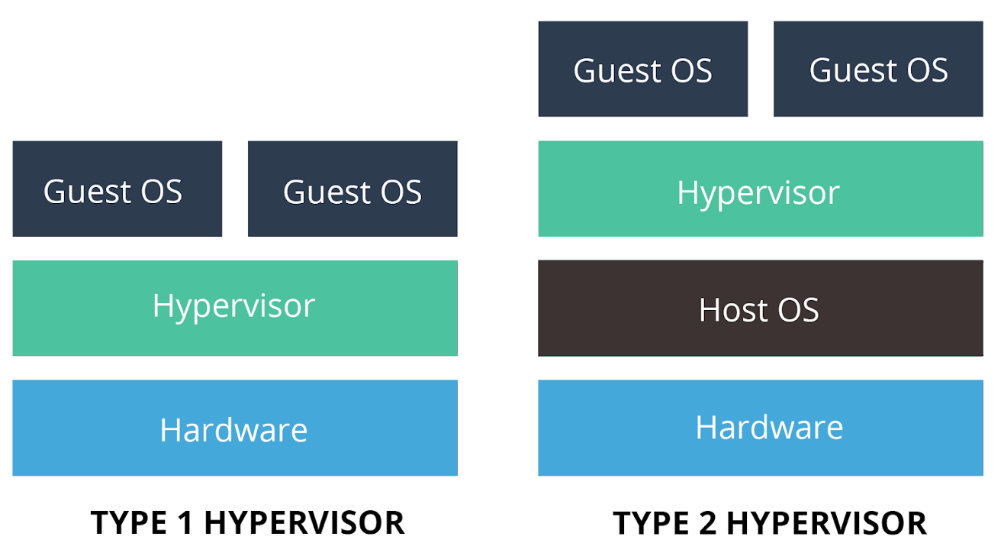
\includegraphics[width=0.6\textwidth]{../imgs/EdA/hipervisor.jpg}
\caption{Tipos de hipervisor}
\label{fig:hipervtypes}
\end{figure}

\subsubsection{VirtualBox}
\subsubsection{VMWare}
\subsection{Virtualización en contenedores}
\subsubsection{LXC}
\subsubsection{Docker}
\section{Tecnologías de aprovisionamiento}
\subsection{Aprovisionamiento estático}
\subsubsection{Docker}
\subsubsection{Vagrant}
\subsection{Aprovisionamiento dinámico}
\subsubsection{Chef}
\subsubsection{Ansible}
\section{Tecnologías de orquestación}
\subsubsection{Docker Compose}
\subsubsection{Kubernetes}
\subsubsection{Terraform}
\subsubsection{A}

	% Diseño
\chapter{Diseño} \label{ch:dis}
  En este capítulo se van a detallar las tecnologías a utilizar, así como las etapas a seguir para la implementación de los escenarios de red. Para ello, se parte de un análisis de los requisitos necesarios a cumplir por el sistema tras el cual se tomarán las decisiones de diseño correspondientes.

\section{Requisitos y decisiones de diseño} \label{sec:req}
  En primer lugar, se han identificado una serie de requisitos que debe cumplir el sistema. Estos se han recogido en la tabla que se muestra a continuación:

  \begin{table}[h]
    \begin{center}
      \begin{tabular}{ | w{c}{1cm} | m{14cm} | }
        \hline\rowcolor{oranget} \textbf{Id} & \textbf{Requisito} \\ \hline
        RD1 & Los escenarios han de estar disponibles en cualquier momento y lugar para su utilización y han de poderse ejecutar en cualquier tipo de sistema. \\ \hline\rowcolor{oranger}
        RD2 & El entorno debe de ser seguro, de forma que no se pongan en riesgo recursos sensibles. \\ \hline
        RD3 & Debe ser escalable, tener un tiempo de arranque reducido y ocupar el menor espacio posible. \\ \hline\rowcolor{oranger}
        RD4 & Ha de ser portable, y debe permitir la configuración de los escenarios para adaptarse a nuevas tendencias o situaciones.  \\ \hline
        RD5 & Es deseable que tanto el despliegue como la conexión y aprovisionamiento sea centralizada. Es decir, que todas las configuraciones que requiera el escenario, tanto las que se lleven a cabo en este trabajo como las futuras (configuración software), se puedan realizar desde el entorno que se va a proporcionar. \\ \hline
      \end{tabular}
      \caption{Requisitos de diseño}
      \label{tab:objs}
    \end{center}
  \end{table}

  Tras el análisis de tecnologías realizado en el capítulo \ref{ch:estado}, podemos determinar aquellas que se adecuan mejor a los requisitos arriba expuestos. Teniendo en cuenta los requisitos \textit{RD1}, \textit{RD2} y \textit{RD3}, se ha decidido que lo mejor es realizar un despliegue en Cloud, para lo cual se ha seleccionado la plataforma Google Cloud Platform. Para orquestar el despliegue de la infraestructura en la nube, cumpliendo con los requisitos \textit{RD3}, \textit{RD4}, y \textit{RD5} se usará Terraform. Finalmente, para la virtualización de los sistemas, en un principio se hará uso de las máquinas virtuales que proporciona Google Cloud. No obstante, en el caso de ser necesarios algunos servicios o funcionalidades concretas, se correrán contenedores Docker dentro de dichas máquinas virtuales, que como se comentó en el estado del arte permiten virtualizar gran cantidad de software de una manera muy sencilla, eficiente, ocupando poco espacio y con un tiempo de arranque muy reducido.

\section{Solución propuesta} \label{sec:sol}
  La solución que se propone es un despliegue en Google Cloud orquestado por Terraform y empleando la tecnología de virtualización Docker.

  El hecho de realizar un despliegue en cloud permite que la infraestructura utilizada para el entrenamiento en ciberseguridad sea completamente independiente de la de la empresa o equipo de quien la usa, lo que proporciona seguridad a las organizaciones que lo usen. 

  Además, esta infraestructura será accesible por cualquiera que tenga autorización, sin importar donde se encuentre. No conlleva costes de operación ni mantenimiento, pues Google se encarga tanto del hardware donde se virtualizan los escenarios como de mantener actualizado el software. Por último es escalable, según se vayan necesitando recursos como almacenamiento o memoria se van asignando sin necesidad de interacción humana, y se paga sólo por los recursos que se usan, lo que supone un gran ahorro en costes.

  A la hora de orquestar el despliegue, Terraform proporciona muchas ventajas. En primer lugar, permite tener en ficheros con una sintaxis muy sencilla la definición de toda la infraestructura. Sólo basta con ejecutar la orden \texttt{terraform apply} para que se despliegue todo de forma automática en la nube. Además los ficheros que describen el estado final deseado de la infraestructura permiten a su vez el uso de ficheros de variables para parametrizar el despliegue y que la configuración sea más modular y sencilla. También permite que los escenarios sean portables, ya que puede ser utilizado con cualquier proveedor de servicios de cloud. De esta forma, si se decide migrar la infraestructura a otro proveedor por cualquier motivo, no habría que reescribir todo el código, como ocurriría con el resto de  herramientas de IaC diseñadas para funcionar con un único proveedor de cloud. Otro aspecto importante es que con cada cambio que se realice en el entorno, la configuración actual se sustituye por una nueva que aplica el cambio y se vuelve a suministrar la infraestructura, lo que se conoce como infraestructura mutable y que facilita su uso junto a un software de control de versiones como GitHub.

  Por último, en cuanto al aprovisionamiento, Terraform permite seleccionar a la hora de definir una instancia la imagen base de esta, bien sea una imagen de las que proporciona Google o una imagen personalizada que hayamos construido y alojado en el propio Google Cloud. Además, en caso de ser necesarias configuraciones extra, Terraform también permite especificar scripts de inicio personalizados que se ejecutan cuando esta se arranca. Estos scripts pueden estar escritos en cualquier lenguaje, y pueden servir para realizar multitud de configuraciones como instalación de paquetes o modificación de ficheros. Un añadido muy interesante que proporciona Terraform es la función \texttt{templatefile}, que recibe como parámetro el path a un script y permite usarlo como una plantilla donde se especifican las variables deseadas. Es mejor verlo en un ejemplo práctico. Imaginemos que tenemos el fichero \texttt{docker.tftpl} con el siguiente contenido: \\

  \begin{lstlisting}[language=Bash, caption=Contenido del fichero docker.tftpl]
  #!/bin/bash
  docker run ${image}\end{lstlisting}

  A la hora de definir la instancia en el fichero de configuración de Terraform, en el campo correspondiente indicamos qué valor queremos que tome esa variable, que como vemos se define con la sintaxis \$\{...\}: \\
  
  \begin{lstlisting}[language=Bash, caption=Extracto de fichero de configuración .tf]
  [...] #Inicio de la definicion de la instancia
   metadata_startup_script=templatefile("templates/docker.tftpl", { image = "nginx" })
  [...] #Fin de la definicion de la instancia\end{lstlisting}

  De esta forma, cuando la instancia se arranque y ejecute el fichero, lo hará sustituyendo “nginx” en el lugar de la variable \texttt{image}. Es importante la extensión \texttt{.tftpl} para que Terraform interprete correctamente las variables. En el caso de no ser necesaria la parametrización del script se pueden enviar directamente scripts en Bash, Python o el lenguaje que se desee haciendo uso de la función \texttt{file}, donde solo sería necesario especificar el path al archivo, a diferencia de la función \texttt{templatefile} que necesita también las variables.

  Como se puede observar, estas funciones proporcionan una gran flexibilidad a la hora de configurar las instancias. Y lo más importante, permiten tener un directorio con archivos de configuración y acceder a ellos desde el mismo fichero donde se configura el despliegue de la infraestructura, de forma que se puede manejar todo de forma centralizada.

\section{Etapas de diseño} \label{sec:etp}
Una vez propuesta la solución, se establecen una serie de etapas de diseño en las que se divide el proceso, siguiendo un orden secuencial que se muestra a continuación:


  \begin{table}[h]
    \begin{center}
      \begin{tabular}{ | w{c}{1cm} | m{14cm} | }
        \hline\rowcolor{oranget} \textbf{Id} & \textbf{Etapa de diseño} \\ \hline
        ED1 & Definición de los escenarios a implementar. \\ \hline\rowcolor{oranger}
        ED2 & Análisis de los escenarios, vector de ataque y conexiones necesarias entre los elementos que lo componen. \\ \hline
        ED3 & Debe ser escalable, tener un tiempo de arranque reducido y ocupar el menor espacio posible. \\ \hline\rowcolor{oranger}
        ED4 & Desarrollo de los ficheros Terraform que permiten la implementación de los escenarios definidos en la nube según el estudio realizado.  \\ \hline
        ED5 & Creación de herramientas que permitan arrancar contenedores Docker, así como realizar algunas pequeñas configuraciones en las instancias y que sirvan como base para la futura configuración de los escenarios. \\ \hline
      \end{tabular}
      \caption{Etapas de diseño}
      \label{tab:objs}
    \end{center}
  \end{table}

  Como resultado de este proceso se obtendrán escenarios de red virtualizados en la nube con todos los elementos y configuraciones necesarias para generar a partir de ellos ejercicios para la formación y entrenamiento en el campo de la ciberseguridad.

	% Desarrollo
\chapter{Desarrollo} \label{ch:des}
En este capítulo se detalla el desarrollo del proyecto siguiendo las etapas de diseño descritas. Se comenzará por la preparación del entorno y posteriormente se describirá la implementación de los escenarios en GCP.

\section{Preparación del entorno} \label{sec:prep}
  Antes de comenzar, es necesario disponer de una cuenta en Google Cloud Platform, así como disponer de un proyecto creado. Para crear un proyecto, basta con seleccionar o crear uno en la página del selector de proyectos de Google Cloud. 

  \begin{figure}[h]
  \centering
  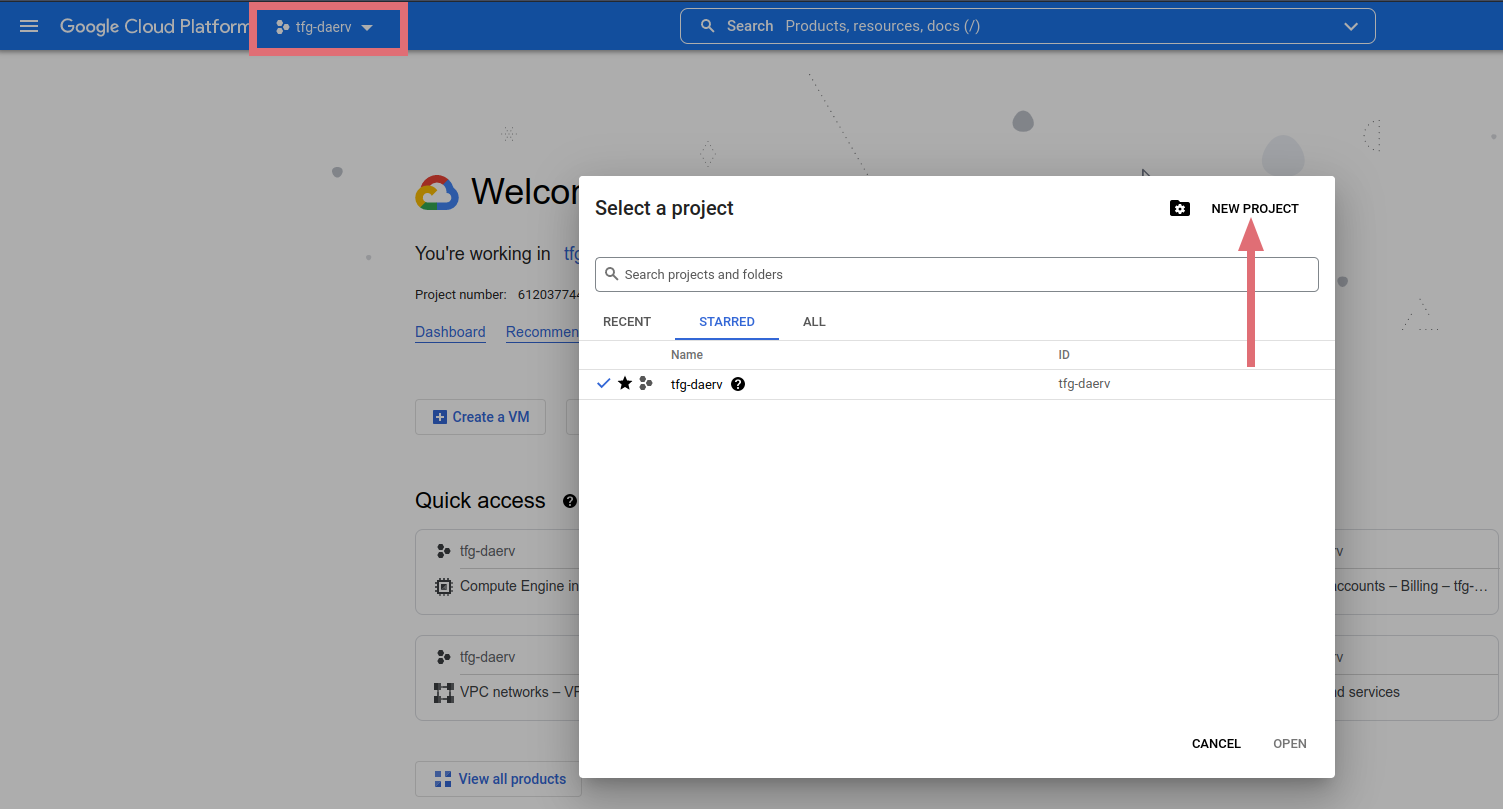
\includegraphics[width=\textwidth]{../imgs/desarrollo/entorno/project.png}
  \caption{Selección de un proyecto en Google Cloud}
  \label{fig:ent1}
  \end{figure}

  Una vez tengamos creada una cuenta y un proyecto en ella, debemos habilitar la API de Google Compute Engine~\cite{des1} para nuestro proyecto en la consola de GCP. También es necesario instalar tanto Terraform como la CLI de Google Cloud. Una vez hecho todo esto, lo primero es autenticarse con GCP. Para ello, basta con ejecutar \texttt{gcloud auth application-default login} en la terminal. Esto nos dirigirá a una página donde podremos iniciar sesión con nuestra cuenta de Google para permitir el acceso a nuestros datos de GCP.

  Para poder realizar peticiones desde Terraform a la API de GCP, también es necesario autenticarse para así probar que somos quien están realizando esas peticiones. Hay varias formas de realizar esta autenticación. Una de ellas es mediante las Cuentas de Servicio de Google Cloud, para la cual hay que seguir los siguientes pasos:

  \begin{enumerate}
    \item En el apartado de Cuentas de Servicio~\cite{des2} de la consola de Google Cloud debemos elegir una cuenta existente, o crear una nueva. A la hora de crearla hay que tener en cuenta que es necesario asignar permisos de edición.
    \item En la sección de claves, debemos generar una clave y descargarla en formato JSON, ponerle un nombre del que nos vayamos a acordar y almacenarla en un lugar seguro. 
    \item Para proporcionarle la clave descargada a Terraform, lo haremos mediante la variable de entorno \texttt{GOOGLE\_APPLICATION\_CREDENTIALS}, asignándole como valor el de la ruta al archivo con la clave ejecutando el siguiente comando:

      \begin{lstlisting}[language=Bash]
	export GOOGLE\_APPLICATION\_CREDENTIALS=\{\{path\}\}\end{lstlisting}

      Para que las credenciales se guarden entre sesiones, es necesario añadir esta línea a un fichero de inicio como \texttt{bash\_profile} o \texttt{bashrc}. Una opción alternativa a la variable de entorno sería proporcionar a Terraform el path a la clave en la configuración del provider, dentro del fichero \texttt{main.tf}.
  \end{enumerate}

  Por último, en el fichero \texttt{.tf} que va a contener todo el código necesario para alcanzar el estado necesario de nuestra infrestructura, hay que configurar el provider de Google. Para ello, en dicho fichero, que normalmente se llama \texttt{main.tf} añadiríamos el código mostrado en la parte inferior, y ejecutaríamos la instrucción \texttt{terraform init} en el mismo directorio donde se encuentra el fichero para que todos e configure correctamente. 

  \begin{lstlisting}[language=Bash]
  provider "google" {
    project = var.project_id
    region  = var.region
    zone    = var.zone
  }\end{lstlisting}

  En este caso, se han utilizado variables almacenadas en el fichero \texttt{variables.tf} para asignar el valor a los parámetros. Además, también cabe mencionar que por comodidad se ha empleado la misma región y zona en todos los escenarios desplegados, ya que el valor de este campo simplemente determina el centro de datos de Google en el que se despliegua la infraestructura.

  Una vez hechas estas configuraciones, ya podemos desarrollar nuestro código Terraform y ordenar que se despliegue la infraestructura en nuestro proyecto simplemente con el comando \texttt{terraform apply}, destruir la infrestructura desplegada con \texttt{terraform destroy} o consultar el estado de los recursos desplegados con la orden \texttt{terraform state list}, entre otras muchas opciones.


\clearpage 
\section{Escenarios de red} \label{sec:scen}
  En esta sección se van a presentar los escenarios de red a simular y se va a desarrollar su implementación en Google Cloud. 

\subsection{Smart Office 1} \label{sec:so1}
\subsubsection{Descripción}
  El escenario \textit{Smart Office 1} simula una oficina que cuenta con una red LAN cableada Ethernet en la que se encuentran conectados los sistemas de la oficina. En dicha oficina, existe un sistema de impresión que permite a los empleados realizar impresiones desde sus ordenadores. Dicho sistema cuenta con uno o varios dispositivos basados en Linux, de los cuales uno es una impresora conectada a un servidor remoto propio de la marca en un entorno Cloud.

  El atacante se encuentra conectado a una red local inalámbrica en la que que también se encuentra el PC de un empleado de la empresa. Dicho empleado está a su vez conectado a la red interna de la empresa mediante una red cableada Ethernet. El objetivo del atacante es lanzar un ataque sobre el servicio de impresión en el que, mediante la modificación del firmware, logre acceder a la red local remota. La impresora no requiere autenticación antes de la actualización de firmware, por tanto esta sería la vulnerabilidad a aprovechar por el atacante.

  \begin{figure}[h]
  \centering
  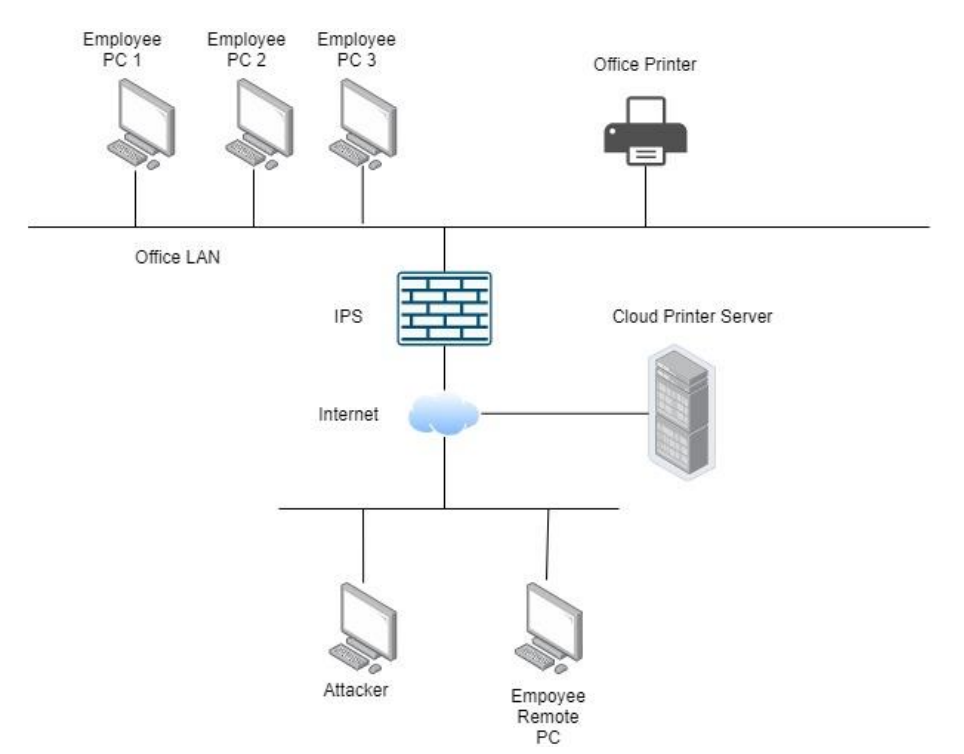
\includegraphics[width=0.7\textwidth]{../imgs/desarrollo/escenarios-de-red/smart-office-1/smart-office-1.png}
  \caption{Topología del escenario Smart Office 1}
  \label{fig:so1-t}
  \end{figure}

  El atacante deberá ganar acceso al equipo del empleado remoto, que es quien tiene conexión con la red interna de la empresa, mediante la explotación de alguno de sus servicios. Una vez hecho esto, recopilaría información referente a la impresora y solicitaría el procesamiento de un documento malicioso, cuyo contenido será enviado y embebido mediante comandos PJL (\textit{Printer Job Languaje}). La aleatoriedad de los comandos haría imposible su detección por parte de los sistemas de seguridad de la empresa, de forma una vez lleguen a la impresora víctima, esta reconocerá que el trabajo de impresión contiene una actualización de firmware válida y permitirá al atacante realizar modificaciones arbitrarias en el área de almacenamiento del firmware. En esta situación, el atacante podrá acceder al servidor de impresión, que actúa como un log descentralizado y podría contener información sensible sobre lo que haya impreso cada empleado.

\subsubsection{Implementación}
  Para la implementación de este escenario se han definido 3 VPCs. Una de ellas representa la oficina interna, donde se ubican 2 instancias de Compute Engine basadas en Linux que representan equipos de empleado y la impresora. Esta red interna está segmentada, es decir, los equipos de empleado se ubican en una LAN diferente a la impresora, siendo una LAN una subred de la VPC. Otra VPC simula la red externa de la empresa, donde se localizan el equipo del atacante y el empleado remoto, ambos en la misma LAN y también basados en Linux. Finalmente, en la tercera VPC se aloja el servidor de impresión.


  \begin{table}[h]
    \begin{center}
      \begin{tabular}{ | m{5cm} | w{c}{3cm} | w{c}{2,5cm} | m{3,75cm} | }
        \hline\rowcolor{oranget} \centering\textbf{VPC} & \textbf{LAN} & \textbf{Rango IP} & \textbf{Equipos} \\ \hline
        \multirow{2}{*}{office-internal-network} & employees-lan & 10.10.10.0/24 & employee-pc-1 employee-pc-2 \\ \cline{2-4}
         & printer-lan & 10.10.20.0/24 & office-printer \\ \hline\rowcolor{oranger} 
        internal-server-network & printer-server-lan & 10.10.30.0/24 & cloud-printer-server \\ \hline
        office-external-network & office-external-lan & 10.10.40.0/24 & employee-remote-pc attacker \\ \hline
      \end{tabular}
      \caption{Estructura del escenario Smart Office 1}
      \label{tab:vpc1}
    \end{center}
  \end{table}


  La conectividad entre las VPCs es la siguiente: se ha establecido un VPC Peering entre las redes externa e interna de la oficina, de forma que se permite la conectividad entre las direcciones IP internas de ambas, lo que simularía la conexión cableada Ethernet previamente mencionada. A su vez, también existe un VPC Peering entre la red interna de la oficina y la red donde se ubica el servidor de impresión, que no es accesible desde internet. De esta forma, los equipos de la red interna de la oficina tendrán conectividad tanto con la red externa como con la red del servidor, mientras entre la red externa y el servidor no existe dicha conectividad.

  En cuanto al acceso a Internet, en cada una de las redes de la oficina se ha desplegado un Cloud Router con su respectivo Cloud NAT, lo que permite que las instancias sin direcciones IP externas que se encuentran en ambas redes puedan crear conexiones salientes a Internet. El servidor es local y por tanto no se ha configurado su acceso a internet. 

  Tal y como se mencionó en el estado del arte, que las instancias tengan conectividad no quiere decir que esta sea efectiva, ya que una de las reglas de FW implícitas rechaza todo el tráfico entrante. Es decir, para que sea posible el intercambio de tráfico deseado, no basta con hacer un peering entre las VPC, sino que hay que definir reglas de FW que permitan o restrinjan el tráfico que se intercambia. Para replicar este escenario, ha sido necesario crear las siguientes:

  \begin{table}[h]
    \begin{center}
      \footnotesize\hspace*{-1.75cm}\begin{tabular}{ | m{2cm} | m{2cm} | w{c}{1,5cm} | m{2cm} | m{2cm} | m{2cm} | w{c}{1,25cm} | w{c}{1,25cm} | }
        \hline\rowcolor{oranget} \centering\textbf{Nombre} & \centering\textbf{VPC} & \textbf{Dirección} & \centering\textbf{Origen} & \centering\textbf{Destino} & \centering\textbf{Protocolos} & \textbf{Puertos} & \textbf{Acción} \\ \hline
        allow-internal & office-internal-network & INGRESS & 10.10.10.0/24 10.10.20.0/24 & \centering- & TCP, UDP, ICMP & 0-65535 & ALLOW  \\ \hline\rowcolor{oranger}
        allow-external & office-external-network & INGRESS & 10.10.40.0/24 & \centering- & TCP, UDP, ICMP & 0-65535 & ALLOW  \\ \hline
        allow-internal-from-external & office-internal-network & INGRESS & employee-remote-pc (IP) & \centering- & TCP, UDP, ICMP & 0-65535 & ALLOW  \\ \hline\rowcolor{oranger}
        allow-external-from-internal & office-external-network & INGRESS & 10.10.10.0/24 10.10.20.0/24 & employee-remote-pc (IP) & TCP, UDP, ICMP & 0-65535 & ALLOW  \\ \hline
        allow-printer-from-server & office-internal-network & INGRESS & 10.10.30.0/24 & printer (IP) & TCP, UDP, ICMP & 0-65535 & ALLOW  \\ \hline\rowcolor{oranger}
        allow-server-from-printer & internal-server-network & INGRESS & printer (IP) & 10.10.30.0/24 & TCP, UDP, ICMP & 0-65535 & ALLOW  \\ \hline 
      \end{tabular}\hspace*{-1.75cm}
      \caption{Reglas de FW del escenario Smart Office 1}
      \label{tab:fw1}
    \end{center}
  \end{table}

  \textbf{allow-internal:} esta regla se aplica a la VPC de la red interna de la oficina. Permite la entrada de tráfico de cualquier protocolo por cualquier puerto siempre y cuando la dirección IP origen se encuentre dentro de la red interna. Al no especificarse destino, aplica a toda la VPC, por lo que en resumen esta regla permite que las instancias de la red interna de la oficina intercambien tráfico entre sí.

  \textbf{allow-external:} análogamente a allow-internal, esta regla permite que el atacante y el empleado remoto intercambien tráfico entre sí, al encontrarse en la misma LAN.

  \textbf{allow-internal-from-external:} se aplica a la red interna de la oficina, de forma que permite la entrada del tráfico procedente únicamente del empleado remoto, ya que es quien está conectado mediante cable a la red interna. Al estar en VPCs distintas, se especifica como origen la IP del empleado remoto. 

  \textbf{allow-external-from-internal:} análogamente a la anterior, se aplica a la red externa de la oficina, y permite la entrada de tráfico procedente tanto de los empleados como de la impresora únicamente hacia empleado remoto, especificando su IP. 

  \textbf{allow-printer-from-server:} se aplica en la red interna de la oficina, permite el tráfico entrante procedente de la LAN donde se encuentra el servidor hacia la impresora.

  \textbf{allow-server-from-printer:} análogamente a la anterior, el servidor sólo acepta tráfico de entrada procedente de la impresora.

  Es necesario puntualizar algunos aspectos acerca de las reglas de FW comunes a todos los escenarios:

  \begin{itemize}
    \item Como se puede apreciar, muchas de las reglas están configuradas para permitir el tráfico de los protocolos TCP, UDP e ICMP por todos los puertos. Por supuesto esto no sería lo óptimo, y cuando se conociese con detalle los servicios y comunicaciones que realiza cada máquina, estas reglas se podrían modificar para  concretar mejor el tráfico que permiten. 

    \item Las reglas de la tabla tienen asignada una prioridad mayor que aquellas reglas que define Google Cloud por defecto. Por tanto, todo el tráfico de entrada a cualquiera de las VPCs que no aparezca definido en la tabla será rechazado. Además, en la tabla sólo se muestran las reglas custom que ha sido necesario crear, por lo que aunque no aparezca, es efectiva la regla por defecto de Google Cloud que permite el tráfico saliente desde cualquier instancia hacia cualquier destino usando cualquier protocolo por cualquier puerto.

    \item A la hora de especificar los orígenes y destinos en Terraform, se hace una referencia al objeto. Es decir, no se especifica como origen un string con el rango de IPs de una subred, si no que se hace referencia al rango de IP que tenga asignada la LAN en ese momento, de forma que si esas IP cambian, no es necesario cambiar la definición de la regla. Esto se puede ver con más detalle en el Anexo \ref{anx:soI}.
  \end{itemize}

  En cuanto al aprovisionamiento, la idea en este escenario sería crear imágenes en Google Cloud a partir de una ISO ya existente, como por ejemplo una imagen basada en Kali Linux para el atacante, o imágenes Windows de usuario para los empleados, ya que las imágenes Windows disponibles en Google Cloud son de Windows Server. Estas imágenes personalizadas se almacenarían en Google Cloud y se podría pasar como parámetro a la instancia a la hora de construirla, como también se puede ver en el Anexo \ref{anx:soI}.

  \clearpage
  \begin{figure}[h]
  \centering
  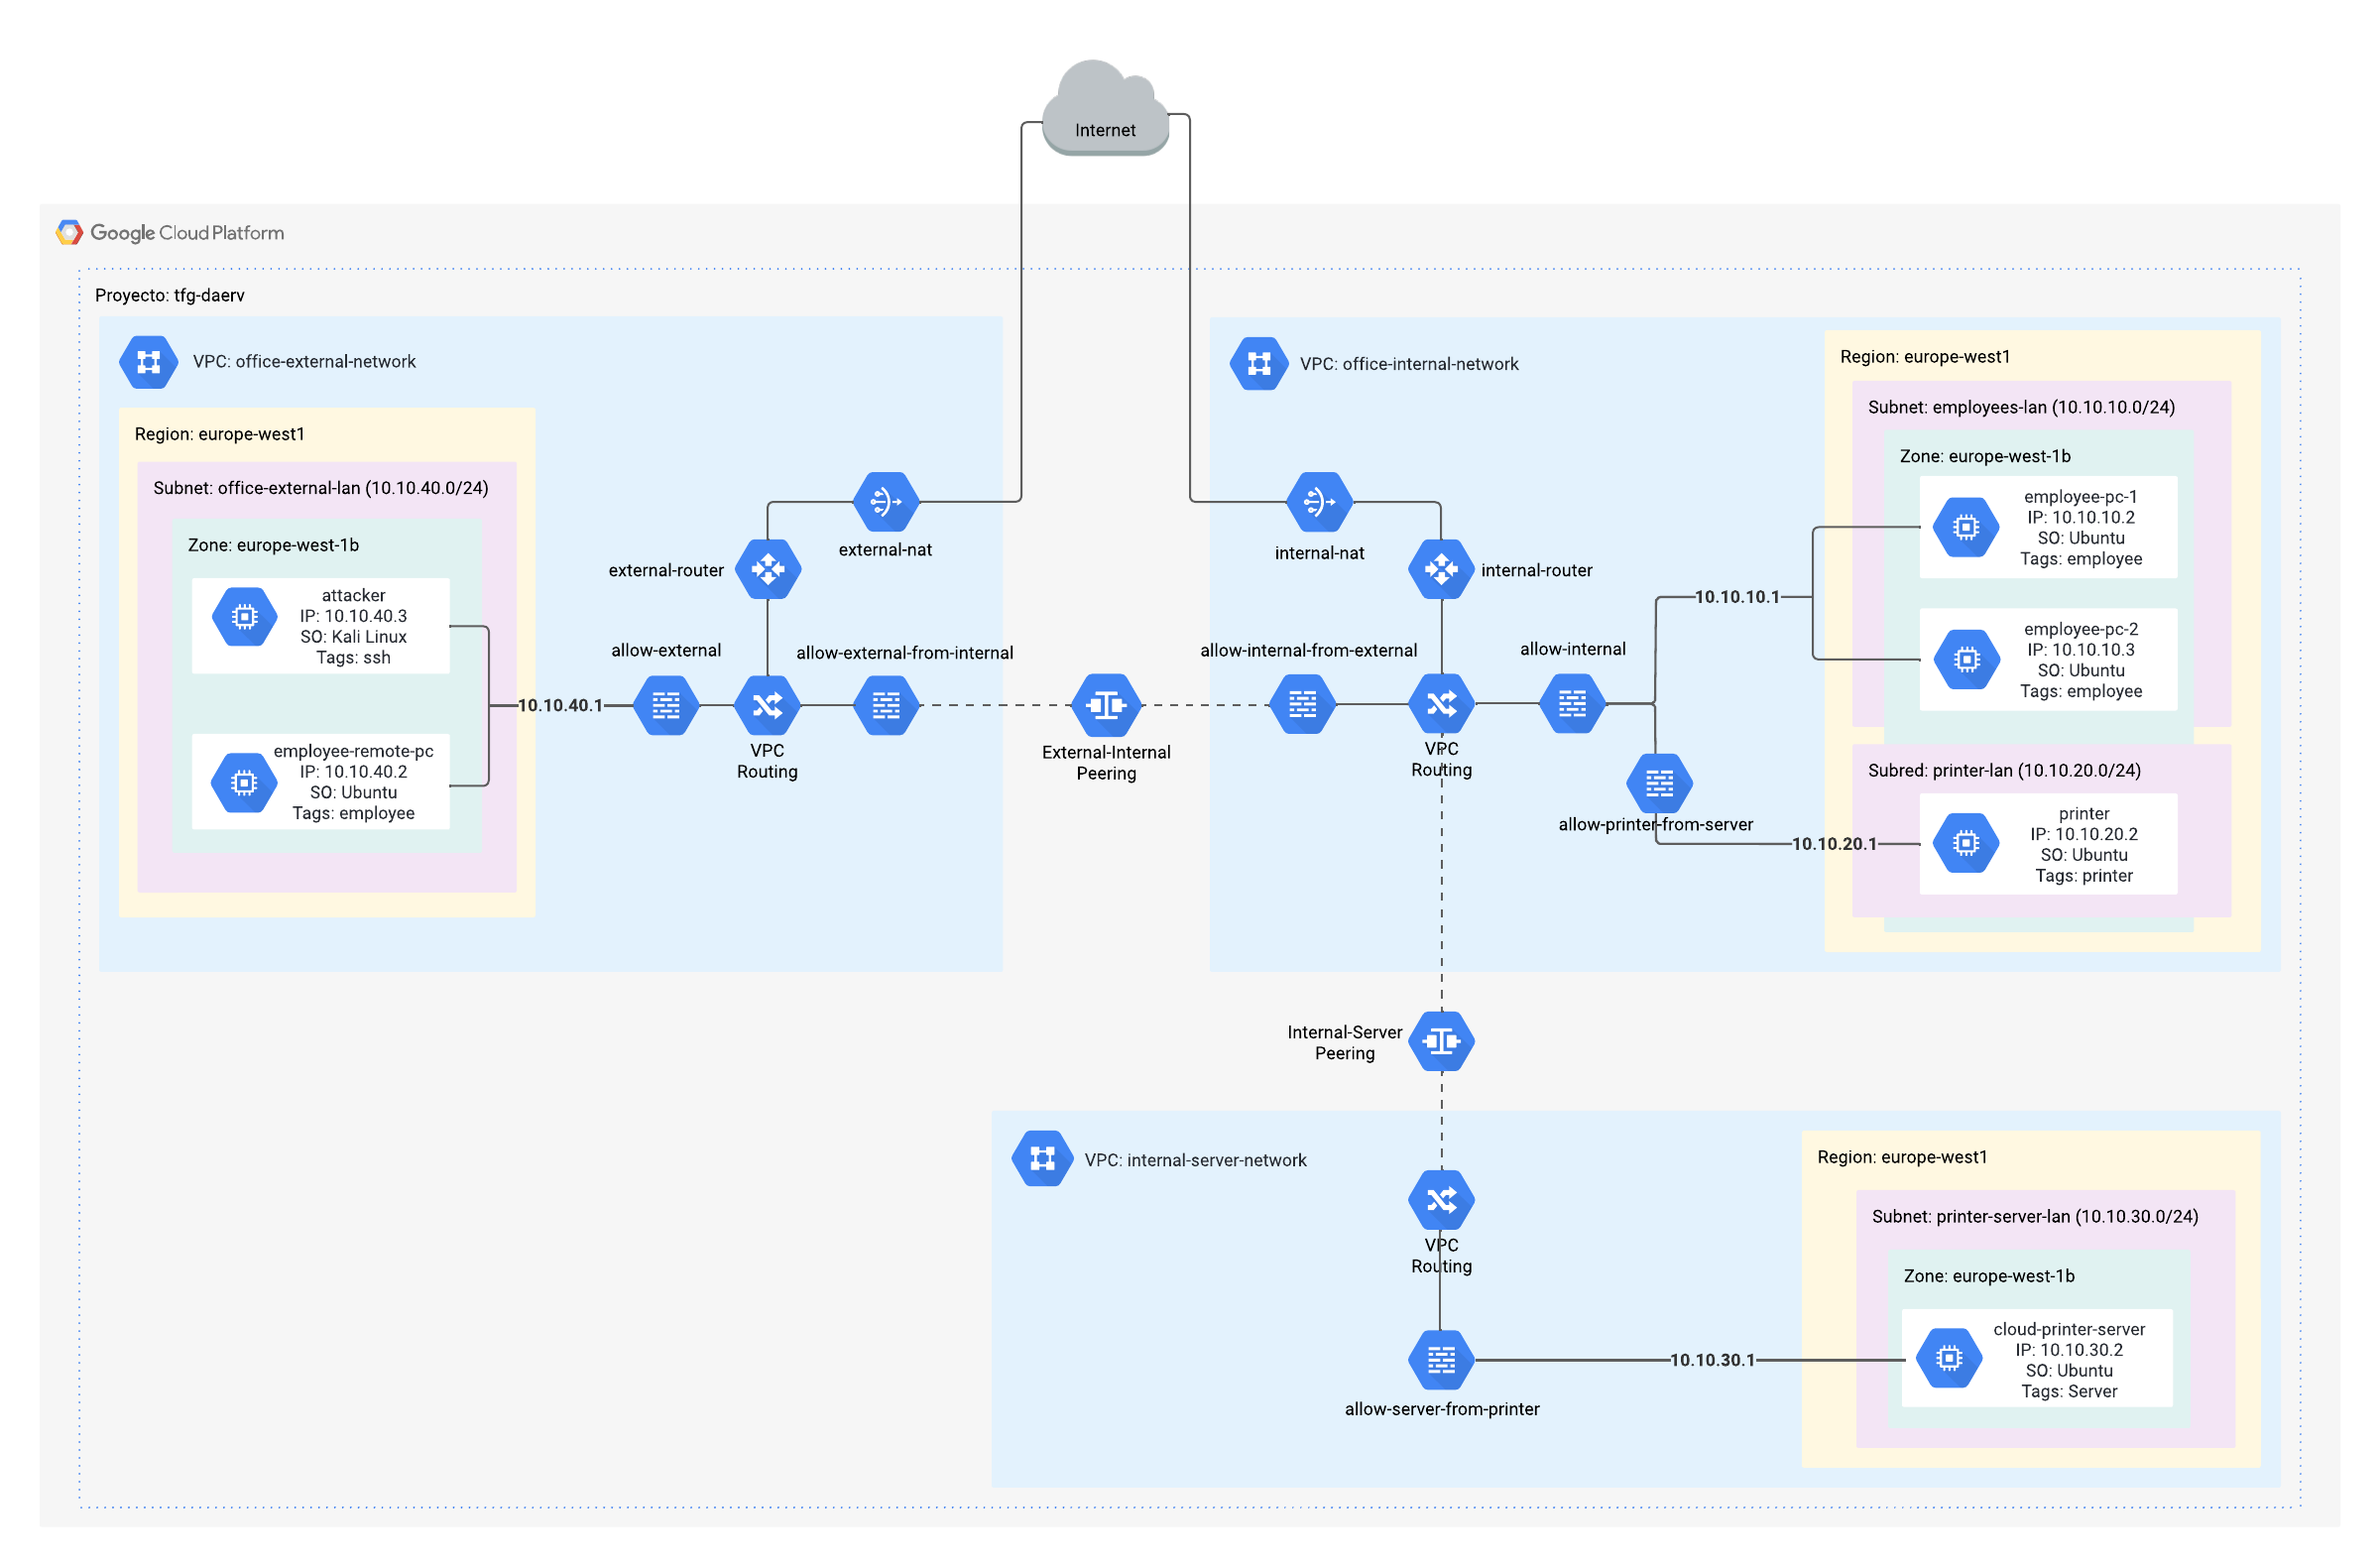
\includegraphics[width=1.45\textwidth, angle=270]{../imgs/desarrollo/escenarios-de-red/smart-office-1/EscenarioSmartOffice1V2.png}
  \caption{Implementación en GCP del escenario Smart Office 1}
  \label{fig:so1-i}
  \end{figure}
  \clearpage 

\subsection{Smart Office 2} \label{sec:so2}
\subsubsection{Descripción}
  El escenario \textit{Smart Office 2} plantea una oficina que cuenta con una red LAN cableada Ethernet en la que se encuentran conectados los sistemas de la oficina. En dicha LAN, existe un sistema de \textit{Smart Speaker} (micrófono y altavoz) que permite a los empleados hacer ciertas tareas utilizando órdenes de voz. Dicho sistema cuenta con uno o varios dispositivos basados en Linux que funcionan como clientes y que escuchan los comandos de voz en la oficina. Estos dispositivos se conectan a un hub interno que, mediante un protocolo IoT permite lanzar comandos básicos a los dispositivos (encendido, apagado, etc) y recibir mensajes de audio capturado a través de los micrófonos. Estos mensajes de audio se cifran y se envían de forma segura desde el hub a un servidor remoto localizado en un entorno Cloud.

  La empresa cuenta con un servicio VPN implementado en el router de entrada a la red LAN que permite a los empleados conectarse a dicha red de forma remota. Existe una vulnerabilidad en el cliente VPN de dicho servicio que permitiría a un atacante robar las credenciales del usuario a través de sus cookies y acceder a la red local. 

  
  El atacante se encuentra conectado a una red LAN en la que también se encuentra el PC de un empleado de la empresa. En dicho PC existe una vulnerabilidad en un servicio de escritorio remoto que permite al atacante acceder a las cookies almacenadas por el cliente VPN y robarlas para suplantar al empleado y acceder a la empresa a través del servicio VPN. Una vez en la red interna, el atacante es capaz de acceder al hub Linux, que se comunica de forma insegura con los dispositivos \textit{Smart Speaker}, siendo capaz de activarlos y desactivarlos arbitrariamente y de recuperar el audio recogido por ellos antes de que se envíe al servidor remoto sin conocimiento de los empleados en la oficina. \\ 

  \begin{figure}[h]
  \centering
  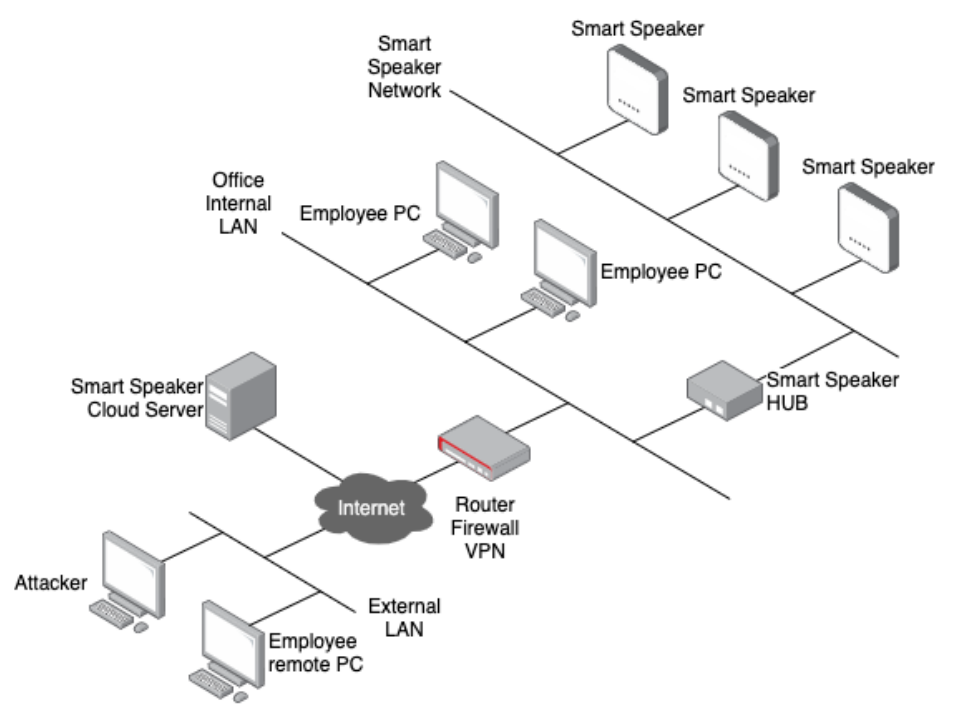
\includegraphics[width=0.7\textwidth]{../imgs/desarrollo/escenarios-de-red/smart-office-2/smart-office-2.png}
  \caption{Topología del escenario Smart Office 2}
  \label{fig:so2-t}
  \end{figure}

\subsubsection{Implementación}
  Este escenario se ha implementado siguiendo la misma base que en el escenario \textit{Smart Office 1}: una VPC una para cada red de oficina  y otra para la red del servidor. Al igual que en el caso anterior, en la red externa se ubica un PC de empleado y el equipo del atacante y en la red del servidor se encuentra el servidor cloud donde se envía el audio recogido por los altavoces inteligentes. La red interna está segmentada en dos LAN, una de ellas con dos PC de empleado y el hub, y la otra con los altavoces inteligentes. Todas los equipos son instancias de Google Compute Engine que usan imágenes Linux, aunque lo ideal sería, como ya se ha comentado, crear una imagen personalizada de Kali Linux para el atacante y una imagen de Windows de escritorio para los empleados. Las VM de la oficina tienen conexión a internet mediante sus respectivos Cloud Nat, mientras que el servidor no está expuesto.

   \begin{table}[h]
    \begin{center}
      \begin{tabular}{ | m{5cm} | w{c}{3cm} | w{c}{2,5cm} | m{3,75cm} | }
        \hline\rowcolor{oranget} \centering\textbf{VPC} & \textbf{LAN} & \textbf{Rango IP} & \textbf{Equipos} \\ \hline
        \multirow{2}{*}{office-internal-network} & office-internal-lan & 10.10.10.0/24 & employee-pc-1 employee-pc-2 smart-speaker-hub \\ \cline{2-4}
         & speakers-lan & 10.10.20.0/24 & smart-speaker-1 smart-speaker-2 smart-speaker-3 \\ \hline\rowcolor{oranger} 
        internal-server-network & speaker-server-lan & 10.10.30.0/24 & smart-speaker-cloud-server \\ \hline
        office-external-network & office-external-lan & 10.10.40.0/24 & employee-remote-pc attacker \\ \hline
      \end{tabular}
      \caption{Estructura del escenario Smart Office 2}
      \label{tab:vpc2}
    \end{center}
  \end{table}

  La interconexión entre las VPC difiere del escenario anterior. Entre la red interna de la oficina y la red del servidor, se mantiene el VPC peering que permite el intercambio de tráfico entre las VPC. En cambio, con el fin de simular la conexión VPN, entre las dos redes de oficina se ha empleado el servicio de Google Cloud llamado Cloud VPN. 

  Cloud VPN permite la conexión segura hacia la red de Google a través de un túnel VPN IPsec. Se ha creado una puerta de enlace VPN en cada una de las VPC, además de un túnel VPN que interconecta ambas puertas de enlace. Una puerta de enlace de VPN encripta el tráfico que viaja entre las dos redes a través de la Internet pública y la otra puerta de enlace de VPN lo desencripta. De esta forma, se protegen los datos mientras viajan por Internet. Cada puerta de enlace tiene una dirección IP pública. Google Cloud ofrece dos tipos de puertas de enlace de Cloud VPN: VPN con alta disponibilidad y VPN clásica. Se han empleado puertas de enlace de alta disponibilidad, dado que proporciona un 99.99\% de esta, además de un encaminamiento más eficiente.

  Pero no sólo ha bastado con crear las puertas de enlace y el túnel. Dado que no se ha entrado en la configuración de las instancias, no está implementado el cliente VPN que permite el intercambio de tráfico entre las puertas de enlace. Como solución temporal, para proporcionar conectividad entre las VPCs se han creado las siguientes rutas estáticas que permiten encaminar los paquetes entre los equipos de las redes de la oficina:

   \begin{table}[h]
    \begin{center}
      \begin{tabular}{ | m{3,5cm} | m{3cm} | w{c}{4cm} | m{3,75cm} | }
        \hline\rowcolor{oranget} \centering\textbf{Nombre} & \centering\textbf{Destino} & \textbf{VPC} & \textbf{Siguiente salto} \\ \hline 
        internal-vpn-route & 10.10.40.0/24 & office-internal-network & internal-vpn-tunnel \\ \hline\rowcolor{oranger}
        external-vpn-route & 10.10.10.0/24 10.10.20.0/24 & office-external-network & external-vpn-tunnel \\ \hline
      \end{tabular}
      \caption{Rutas del escenario Smart Office 2}
      \label{tab:rut2}
    \end{center}
  \end{table}

  Una vez existe la conectividad deseada entre los equipos, es necesario aceptar o denegar el tráfico entrante o saliente. Las reglas de firewall creadas se recogen a continuación:

  \begin{table}[h]
    \begin{center}
      \footnotesize\hspace*{-1.75cm}\begin{tabular}{ | m{2cm} | m{2cm} | w{c}{1,5cm} | m{2cm} | m{2cm} | m{2cm} | w{c}{1,25cm} | w{c}{1,25cm} | }
        \hline\rowcolor{oranget} \centering\textbf{Nombre} & \centering\textbf{VPC} & \textbf{Dirección} & \centering\textbf{Origen} & \centering\textbf{Destino} & \centering\textbf{Protocolos} & \textbf{Puertos} & \textbf{Acción} \\ \hline
        allow-internal & office-internal-network & INGRESS & 10.10.10.0/24 & \centering- & TCP, UDP, ICMP & 0-65535 & ALLOW  \\ \hline\rowcolor{oranger}
        allow-external & office-external-network & INGRESS & 10.10.40.0/24 & \centering- & TCP, UDP, ICMP & 0-65535 & ALLOW  \\ \hline
        allow-hub-from-speakers & office-internal-network & INGRESS & speaker (tag) & speaker-hub (tag) & TCP, UDP, ICMP & 0-65535 & ALLOW  \\ \hline\rowcolor{oranger}
        allow-speakers-from-hub & office-internal-network & INGRESS & speaker-hub (tag) & speaker (tag) & TCP, UDP, ICMP & 0-65535 & ALLOW  \\ \hline
        allow-internal-from-external & office-internal-network & INGRESS & employee-remote-pc (IP) & \centering- & TCP, UDP, ICMP & 0-65535 & ALLOW  \\ \hline\rowcolor{oranger}
        allow-external-from-internal & office-external-network & INGRESS & 10.10.10.0/24 & employee-remote-pc (IP) & TCP, UDP, ICMP & 0-65535 & ALLOW  \\ \hline
        allow-hub-from-server & office-internal-network & INGRESS & 10.10.30.0/24 & smart-speaker-hub (IP) & TCP, UDP, ICMP & 0-65535 & ALLOW  \\ \hline\rowcolor{oranger}
        allow-server-from-hub & internal-server-network & INGRESS & smart-speaker-hub (IP) & 10.10.30.0/24 & TCP, UDP, ICMP & 0-65535 & ALLOW  \\ \hline 
      \end{tabular}\hspace*{-1.75cm}
      \caption{Reglas de FW del escenario Smart Office 2}
      \label{tab:fw2}
    \end{center}
  \end{table}

  Se aprecia que las reglas de FW son prácticamente iguales a las del escenario Smart Office 1. La diferencia principal radica en que en este escenario, la regla allow-internal tiene como origen sólo el rango 10.10.10.0/24, lo que permite el intercambio de tráfico únicamente entre los ordenadores de empleado y el hub. Esto se debe a que la conexión con los altavoces está restringida, de forma que sea sólo el hub quien pueda recibir y enviar tráfico desde y hacia los altavoces, de ahí la necesidad de las reglas allow-speakers-from-hub y allow-hub-from-speakers, que limitan dicho tráfico haciendo uso de las etiquetas de red de cada instancia (recordemos que, al encontrarse en la misma VPC, es más cómodo usar los tags que las direcciones IP). Por la misma razón, la regla allow-external-from-internal también admite como IP origen únicamente la de la LAN interna, puesto que al empleado externo tampoco le está permitida la conexión directa con los altavoces.

  \clearpage
  \begin{figure}[h]
  \centering
  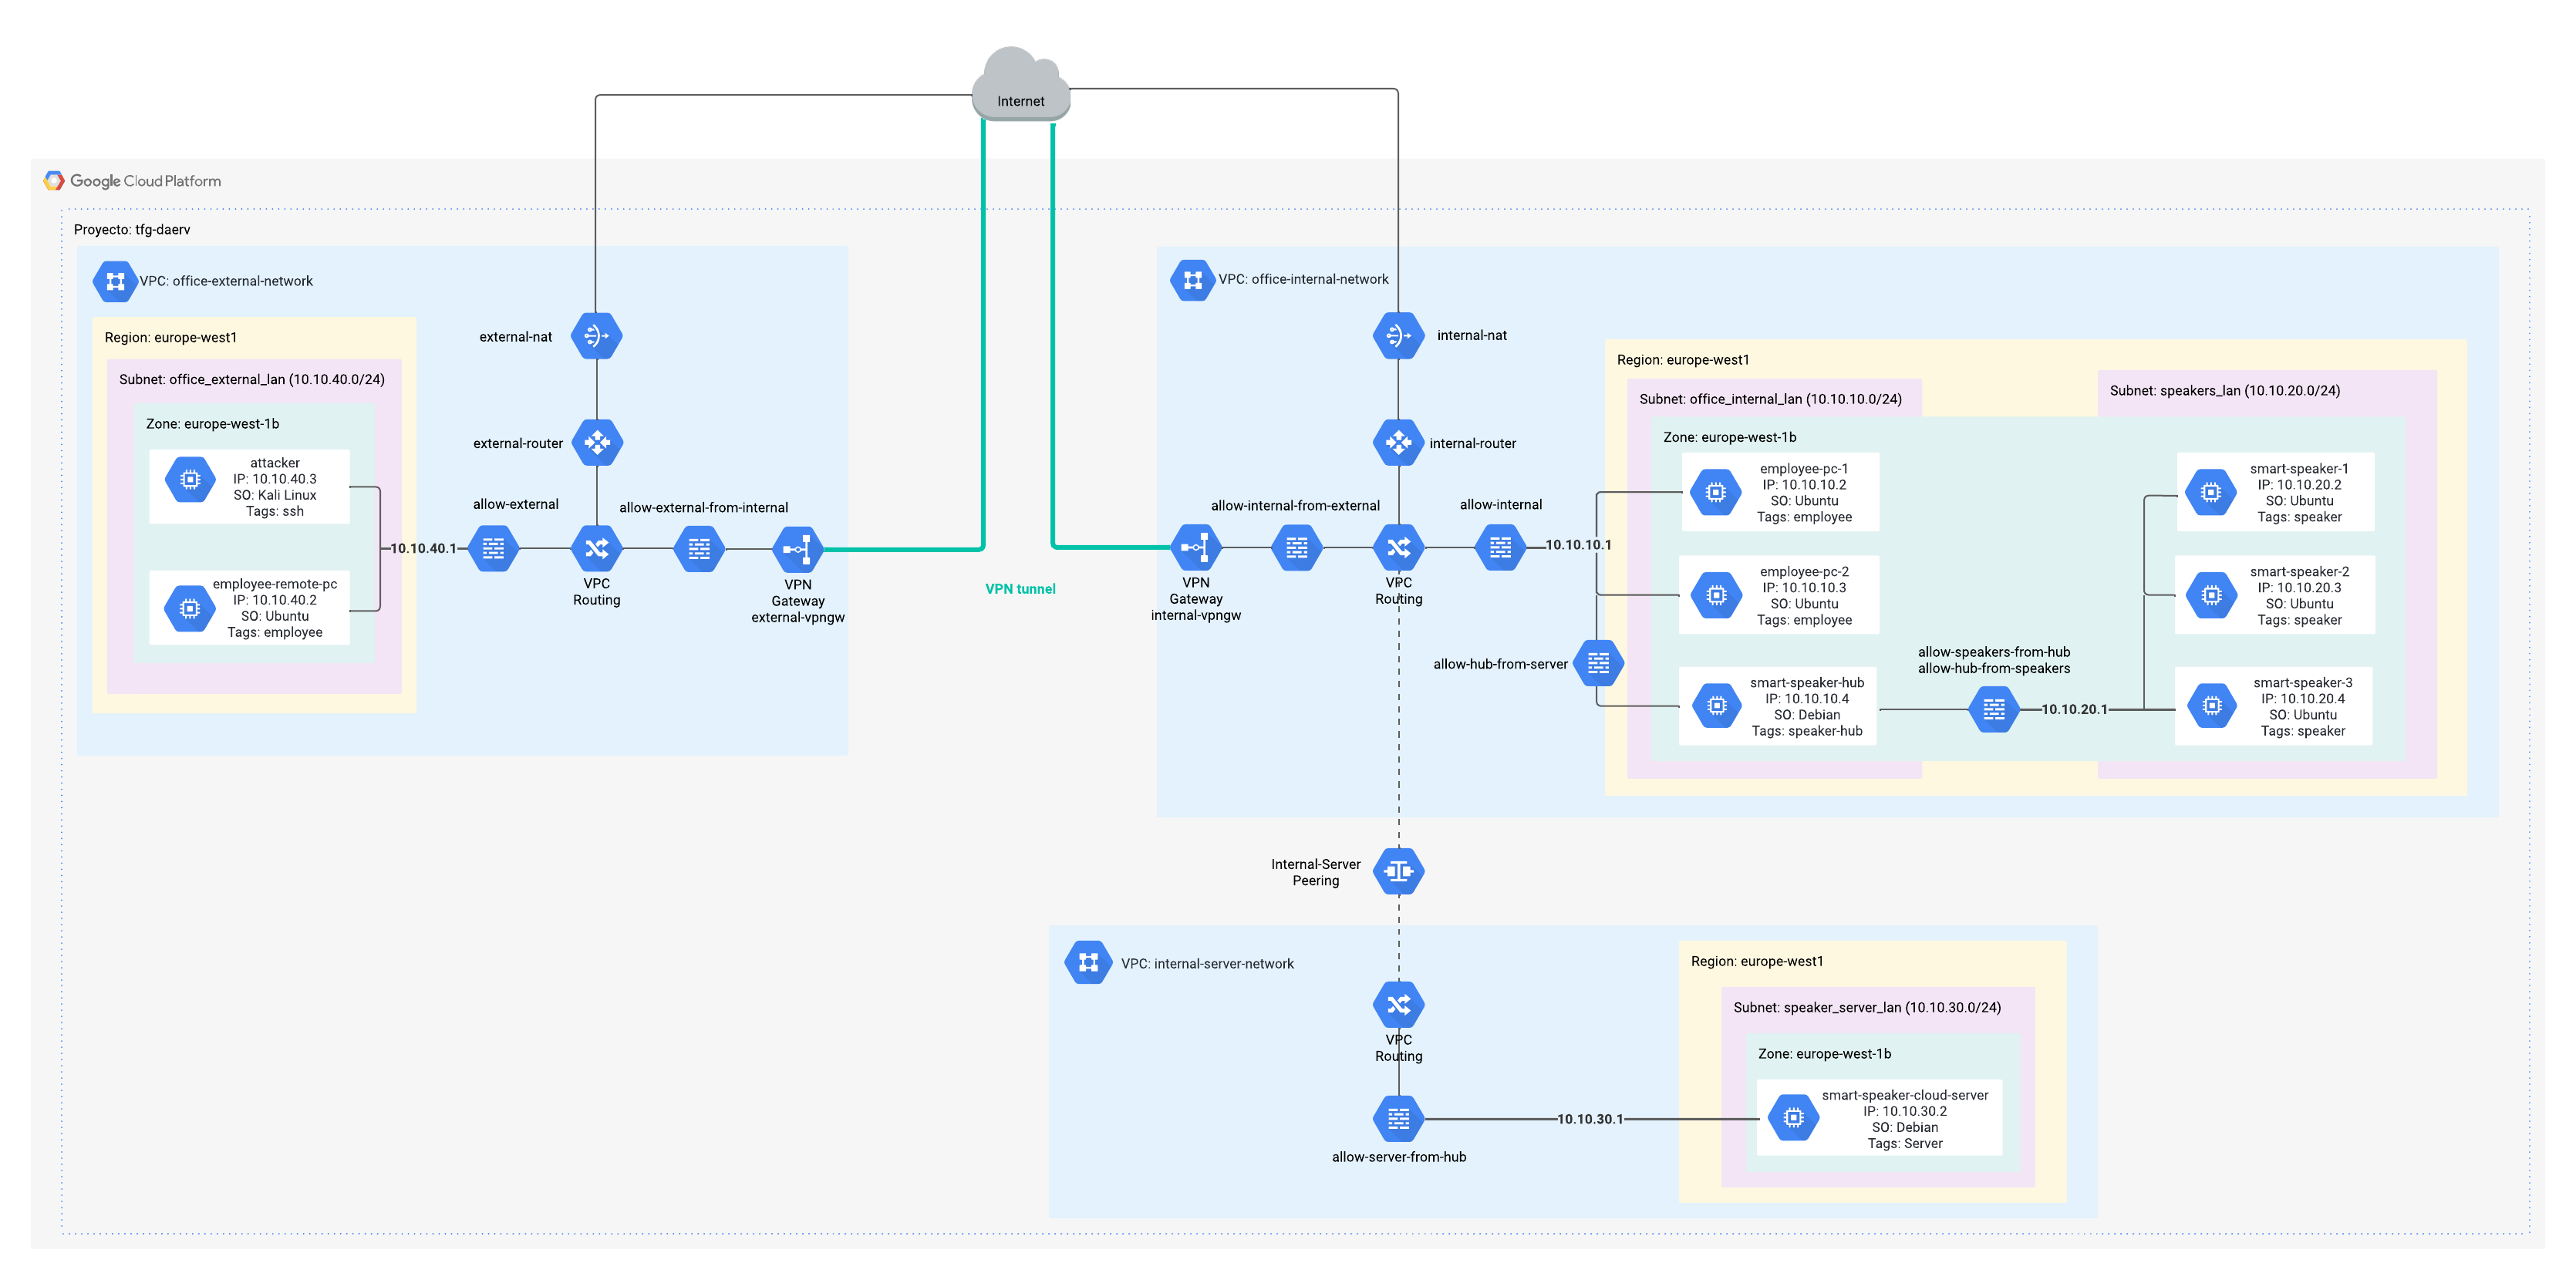
\includegraphics[width=1.45\textwidth, angle=270]{../imgs/desarrollo/escenarios-de-red/smart-office-2/EscenarioSmartOffice2V2.png}
  \caption{Implementación en GCP del escenario Smart Office 2}
  \label{fig:so2-i}
  \end{figure}
  \clearpage

\subsection{Smart Home} \label{sec:sh}
\subsubsection{Descripción}
  Este escenario representa una red de tipología \textit{Smart Home}, con un Access Point (AP) inalámbrico que ofrece conectividad a los dispositivos IoT de la casa. Además, la casa inteligente está controlada por un \textit{Homematic Central Control Unit} (CCU2) que expone la vulnerabilidad CVE-2019-14423 en un addon del firmware, lo que permite la ejecución remota de código (RCE) de forma que atacantes remotos autentificados podrían ejecutar comandos del sistema como root de forma remota a través de una simple petición HTTP.

  Además, otros dos dispositivos de la red exponen vulnerabilidades. En concreto, una bombilla inteligente (Signify Phillips Taolight Smart Wi-Fi Wiz Connected LED Bulb) permite a los usuarios remotos controlar su funcionamiento (CVE-2019-18980) y una cámara IP (Cisco Video Surveillance 8000 Series IP Cameras) podría permitir a un atacante adyacente no autenticado hacer que una cámara IP afectada se recargue (CVE-2021-1131). 

  El atacante tiene acceso a la red y puede explotar cualquiera de las tres vulnerabilidades mencionadas, que se explican con mayor detalle a continuación:

  La versión de firmware 2.31.25 del Homematic CCU2 muestra graves fallos de seguridad que permiten a un atacante obtener acceso completo al sistema y potencialmente también a los dispositivos periféricos conectados a través de comandos de shell que utilizan indebidamente la vulnerabilidad RCE. En cuanto a la bombilla, el modelo mencionado hace uso de una API no protegida (no hay autenticación ni cifrado para utilizarla) que permite que cualquiera pueda encenderla, apagarla o cambiar su brillo de forma remota. El único requisito es que el atacante tenga acceso a la red de la bombilla. Finalmente, en las cámaras IP de la serie 8000 de Cisco Video Surveillance, una vulnerabilidad en la implementación del protocolo Cisco Discovery permite que, enviando un paquete malicioso de Cisco Discovery Protocol a una cámara afectada, el atacante pueda realizar un ataque DoS al provocar que la cámara se recargue inesperadamente. 

  \begin{figure}[h]
  \centering
  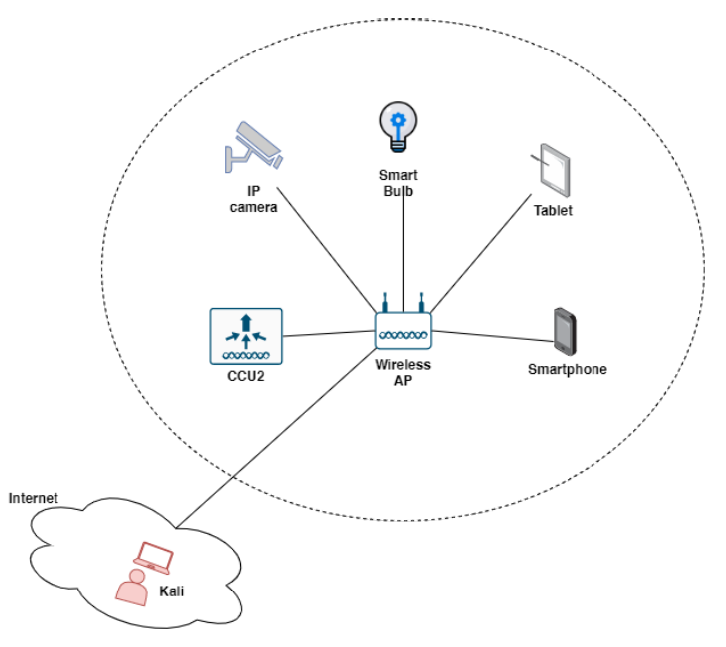
\includegraphics[width=0.5\textwidth]{../imgs/desarrollo/escenarios-de-red/smart-home/smart-home.png}
  \caption{Topología del escenario Smart Home}
  \label{fig:sh-t}
  \end{figure}

\subsubsection{Implementación}
  Para la simulación del escenario \textit{Smart Home} se han desplegado dos VPCs. La primera VPC representa la red local de la casa, que contiene 6 instancias Linux, que se corresponden con los dispositivos conectados a ella. La segunda VPC contiene únicamente el equipo del atacante, y su única función es la de brindarle a este acceso a la red de la casa, para lo cual se ha establecido un VPC peering entre ambas VPC. De esta forma, el atacante tiene acceso a la red local de la casa, lo que le permitirá explotar las vulnerabilidades que se han presentado anteriormente.

  \begin{table}[h]
    \begin{center}
      \begin{tabular}{ | m{5cm} | w{c}{2cm} | w{c}{2,5cm} | m{4,75cm} | }
        \hline\rowcolor{oranget} \centering\textbf{VPC} & \textbf{LAN} & \textbf{Rango IP} & \textbf{Equipos} \\ \hline
        smart-home & home-lan & 10.10.10.0/24 & wireless-ap, tablet, ccu2, ip-camera, smart-bulb, smartphone \\ \hline\rowcolor{oranger}
        attacker & attacker-lan & 10.10.20.0/24 & attacker \\ \hline 
        \end{tabular}
      \caption{Estructura del escenario Smart Home}
      \label{tab:vpc3}
    \end{center}
  \end{table}

  En este caso, en la VPC \textit{smart-home} no se ha empleado Cloud NAT para proporcionar acceso a internet a las instancias. A fin de que la representación de la casa sea lo más realista posible, lo que se ha hecho en esta VPC ha sido asignar una IP pública dinámica a la instancia wireless-ap (las instancias con una IP pública tienen acceso a Internet) y configurarla como un proxy, de forma que el resto de periféricos que se encuentran en la LAN de la casa accedan a internet a través de esta, sin necesidad de Cloud NAT ni de una IP pública en cada uno. De esta forma, se persigue simular el funcionamiento habitual de un router, en el que el proveedor de servicios de Internet (ISP) le asigna una IP pública dinámica que es usada por todos los dispositivos de la casa para acceder a Internet. 

  Para lograr esta configuración, se han creado dos template-files de Terraform. Realmente son scripts en Bash, pero se usa el formato \texttt{.tftpl} de Terraform para poder interpretar objetos de Terraform y usarlos como variables. El primero es \texttt{proxy-config.tftpl}. Este script es llamado en el proceso de creación de la instancia wireless-ap y se encarga de configurarla como un proxy de acceso a Internet. El contenido del script está disponible en el ANEXO. Básicamente se realiza una instalación de Squid y se configura el rango de direcciones IP privadas origen de las que el proxy debe aceptar conexiones para así permitir su acceso a Internet. Este rango de direcciones se le pasa como parámetro al script a la hora de invocarlo, y dicho parámetro es una referencia al rango de IPs que tenga asignada la LAN de la casa en ese momento, de modo que, si en algún momento se decidiera cambiar el rango de direcciones IP en el fichero \texttt{variables.tf}, esto no afectaría al script en absoluto.

  Para aprovisionar los periféricos conectados a la LAN de la casa se ha creado el script \texttt{docker-proxy-config.tftpl}, que instala Docker en las máquinas basadas en Linux en función de la distribución elegida. El script recibe como parámetro una referencia a la IP privada de la instancia configurada como proxy. Esta IP se utiliza para definir las variables \texttt{HTTP\_PROXY} y \texttt{HTTPS\_PROXY}, necesarias para el acceso a Internet. Una vez hecho esto, se emplean comandos Unix para determinar con qué distribución de Linux se está tratando (Debian o Ubuntu), ya que la instalación de Docker difiere en función de cual sea. Conocida la distribución, se hace uso de las variables del proxy para acceder a Internet y descargar Docker. Por último, una vez se ha instalado Docker, se arranca el contenedor deseado según una imagen, unos argumentos y un tag que también se le pasan como parámetro al script a la hora de invocarlo y que permiten arrancar.

  Cabe mencionar que la instalación de Docker no es necesaria para todos los periféricos. En el caso del ccu2 o la bombilla es una buena opción ya que existen imágenes Docker que simulan el comportamiento de estos dispositivos y que por tanto nos permitirían configurar el escenario de la forma deseada de una forma muy sencilla gracias al script. Por el contrario, para el smartphone y la tablet, que son equipos de usuario (y no un servicio) y tendrían un papel secundario en el escenario como puede ser la generación de tráfico, lo más adecuado sería construir una imagen personalizada basada en AndroidOS y desplegar las instancias a partir de ella, indicándolo en el fichero \texttt{main.tf}.

  En cuanto al intercambio de tráfico, solo ha sido necesaria la definición de dos reglas:

  \textbf{allow-internal:} esta regla se aplica a la VPC de la casa y permite el intercambio de tráfico entre los equipos de la LAN (acepta tráfico de todos los protocolos por todos los puertos siempre y cuando la IP origen esté dentro de la LAN, y al no especificarse destino se aplica a todas las instancias de la VPC). 

  \textbf{allow-home-from-attacker:} permite la entrada de tráfico procedente de la VPC del atacante hacia la VPC de la casa. Como se puede observar, no existe la regla \textit{allow-attacker-from-home}, ya que tal y como se comentó en el estado del arte, la regla \textit{allow-home-from-attacker} permite el tráfico de retorno hacia el atacante asociado a ella, lo que no hace necesaria la existencia de una regla que permita que el atacante acepte tráfico procedente de la casa.


  \begin{table}[h]
    \begin{center}
      \footnotesize\hspace*{-1.75cm}\begin{tabular}{ | m{2cm} | m{2cm} | w{c}{1,5cm} | m{2cm} | m{2cm} | m{2cm} | w{c}{1,25cm} | w{c}{1,25cm} | }
        \hline\rowcolor{oranget} \centering\textbf{Nombre} & \centering\textbf{VPC} & \textbf{Dirección} & \centering\textbf{Origen} & \centering\textbf{Destino} & \centering\textbf{Protocolos} & \textbf{Puertos} & \textbf{Acción} \\ \hline
        allow-internal & smart-home & INGRESS & 10.10.10.0/24 & \centering- & TCP, UDP, ICMP & 0-65535 & ALLOW  \\ \hline\rowcolor{oranger}
        allow-home-from-attacker & smart-home & INGRESS & 10.10.20.0/24 & \centering- & TCP, UDP, ICMP & 0-65535 & ALLOW  \\ \hline
      \end{tabular}\hspace*{-1.75cm}
      \caption{Reglas de FW del escenario Smart Home}
      \label{tab:fw3}
    \end{center}
  \end{table}

  \clearpage
  \begin{figure}[h]
  \centering
  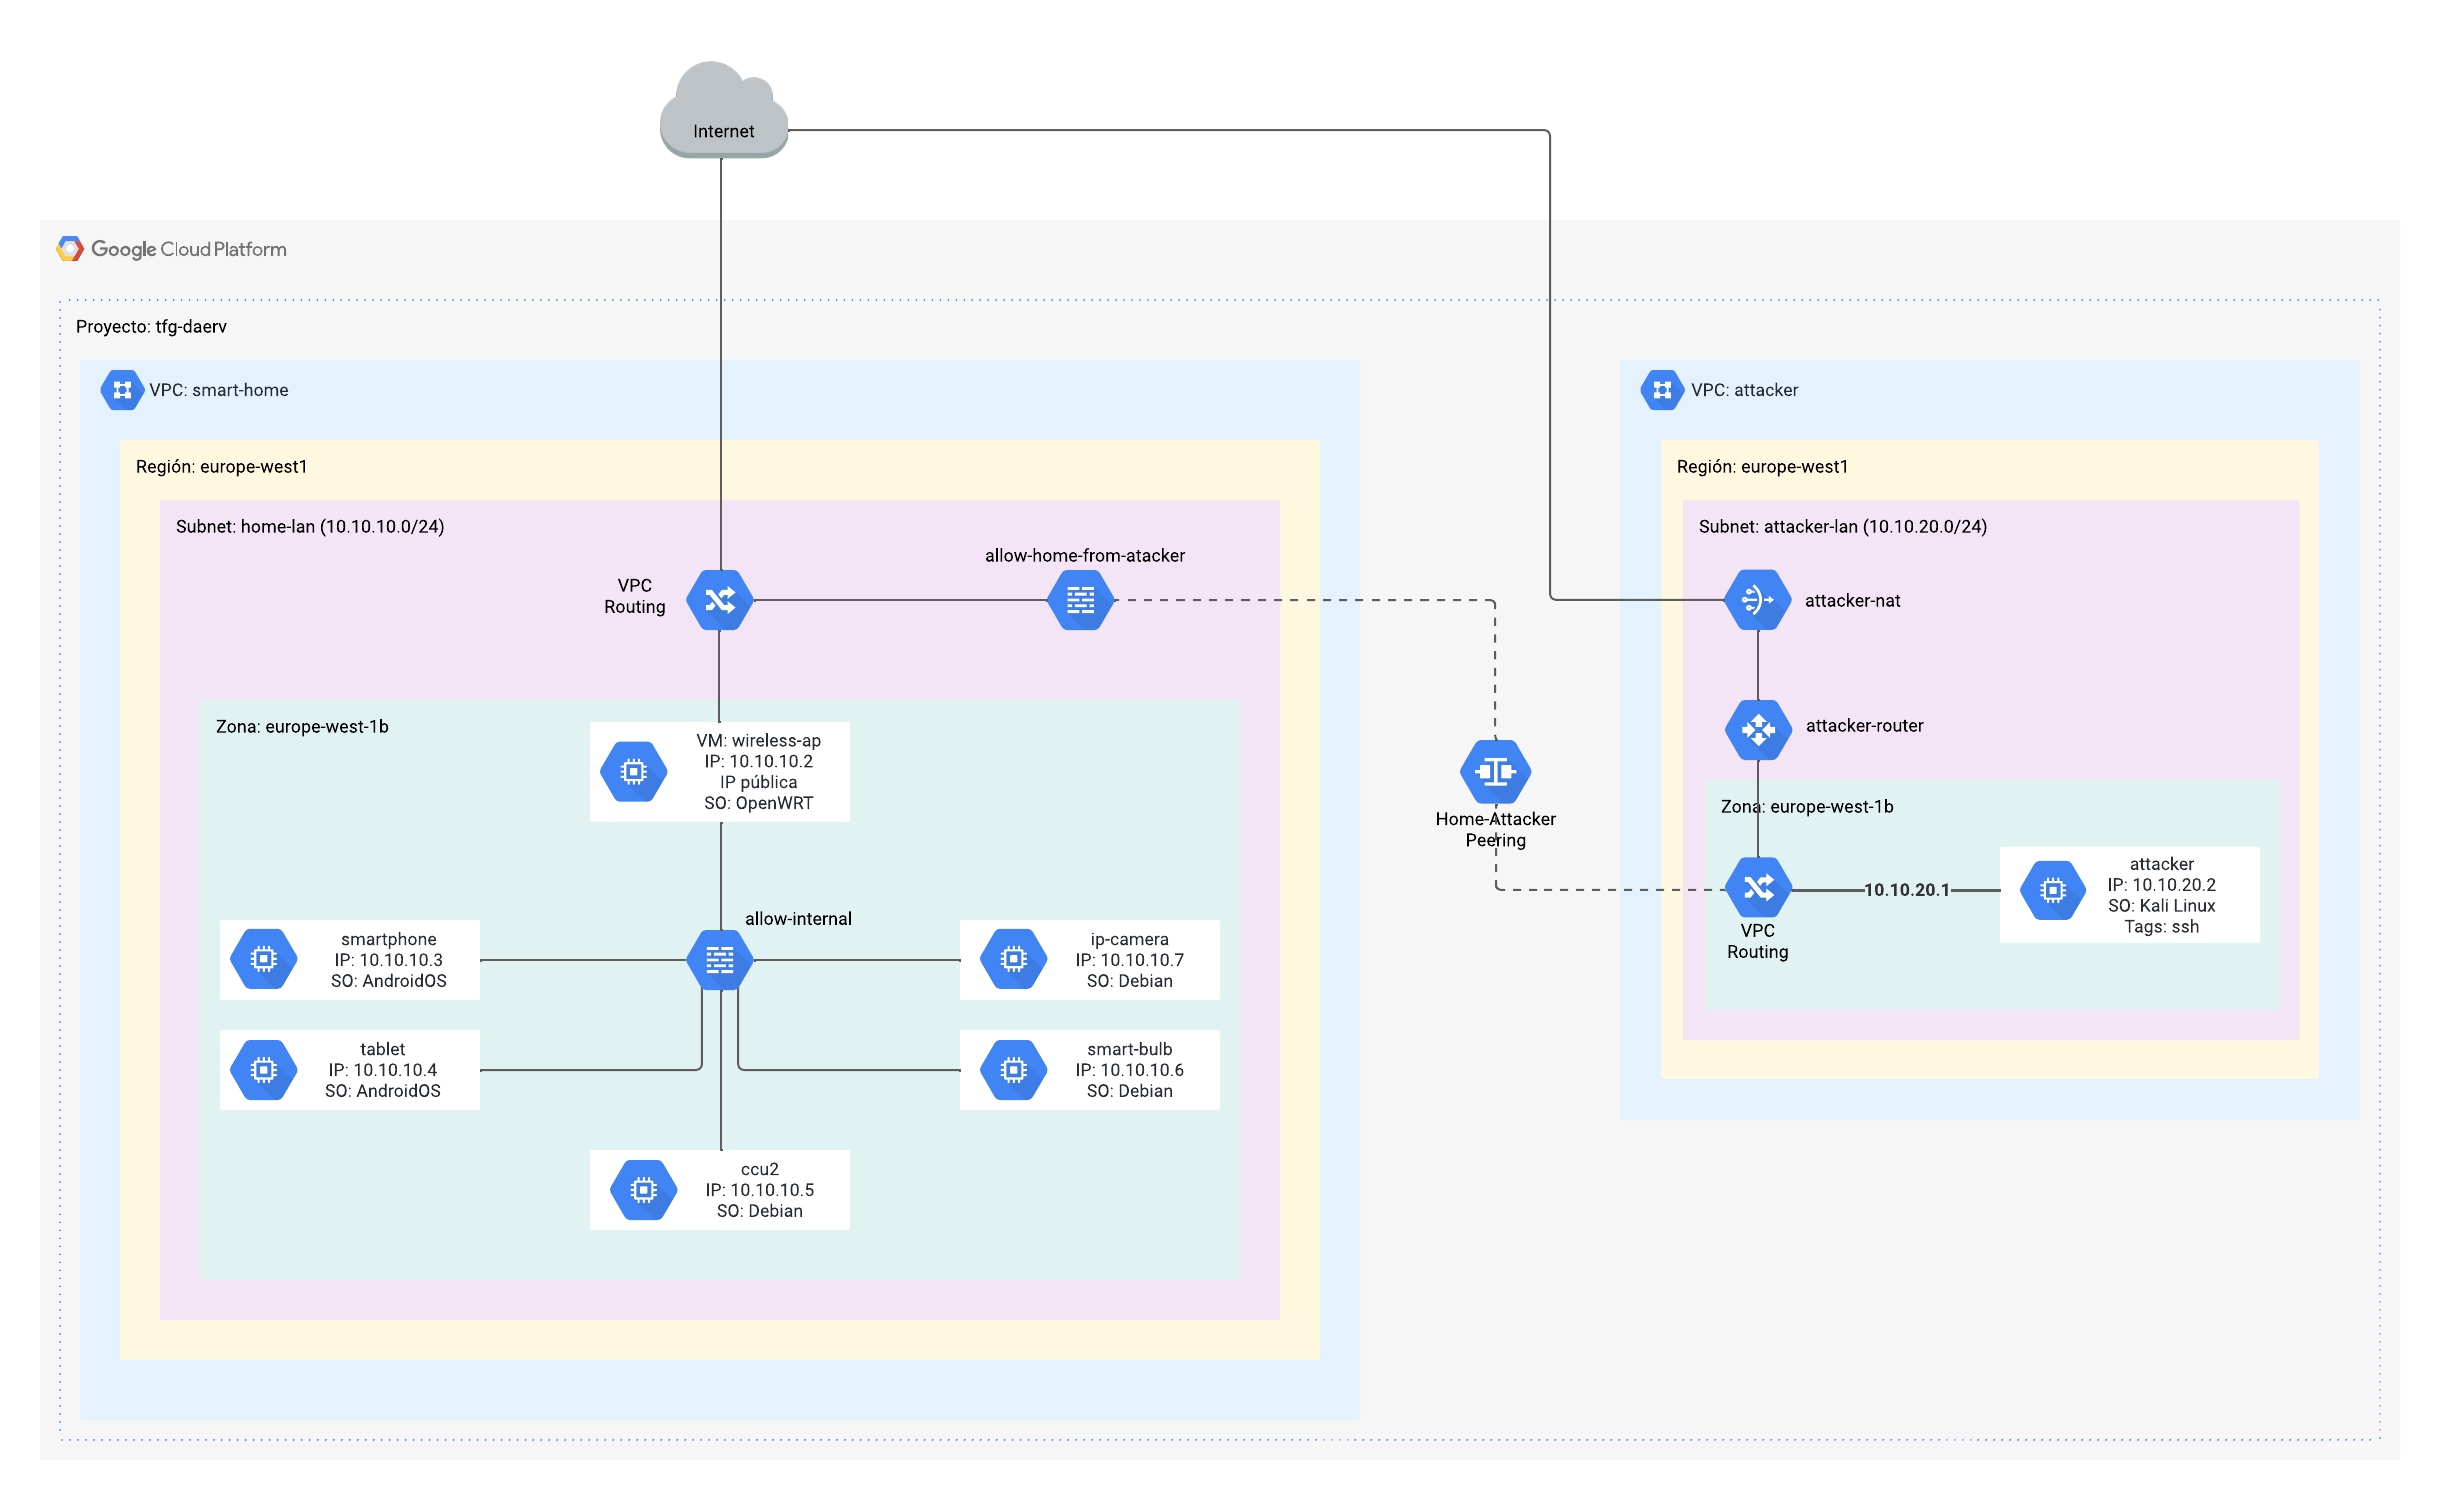
\includegraphics[width=1.45\textwidth, angle=270]{../imgs/desarrollo/escenarios-de-red/smart-home/EscenarioSmartHome.png}
  \caption{Implementación en GCP del escenario Smart Home}
  \label{fig:sh-i}
  \end{figure}
  \clearpage

\subsection{SCADA} \label{sec:sh}
\subsubsection{Descripción}
  El sistema SCADA es una herramienta de automatización y control industrial utilizada en los procesos productivos que puede controlar, supervisar, recopilar datos, analizar datos y generar informes a distancia mediante una aplicación informática. Su principal función es la de evaluar los datos con el propósito de subsanar posibles errores. Los sistemas SCADA son cruciales para las empresas industriales, ya que ayudan a mantener la eficiencia, procesar los datos para tomar decisiones más inteligentes y comunicar los problemas del sistema para reducir el tiempo de inactividad.

  Este escenario resulta de la agrupación de aplicaciones informáticas instaladas en un ordenador denominado Máster o MTU, destinado al control automático de una actividad productiva a distancia que está interconectada con otros instrumentos llamados de campo como son los autómatas programables (PLC) y las unidades terminales remotas (RTU). El HMI es la interfaz que conecta al hombre con la maquina presentando los datos del proceso ante el operario mediante un sistema de monitoreo. Además, controla la acción a desarrollar a través de una pantalla.

  \begin{figure}[h]
  \centering
  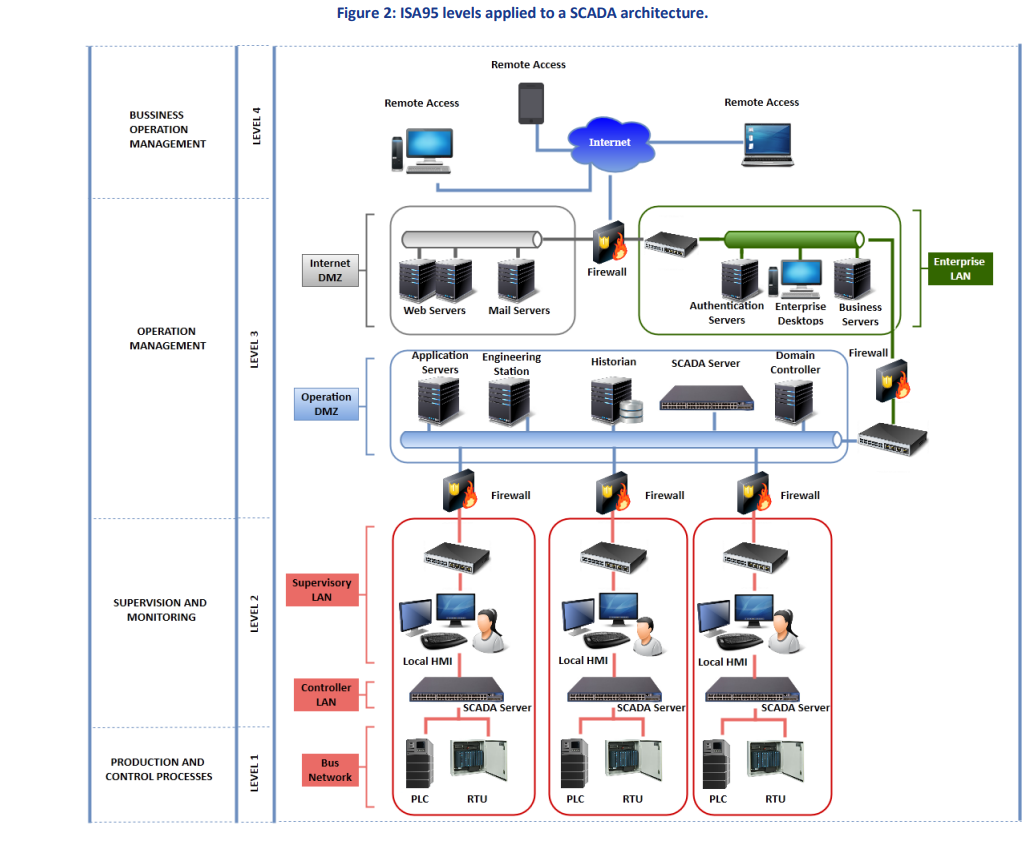
\includegraphics[width=0.9\textwidth]{../imgs/desarrollo/escenarios-de-red/SCADA/SCADA_Network_2.PNG}
  \caption{Topología del escenario SCADA}
  \label{fig:scada-t}
  \end{figure}
  
  En la zona DMZ de la subred IT se encuentra un servidor web público que corre un Nginx desactualizado vulnerable a \textit{integer overflow} (CVE-2017-7529) y que permitiría al atacante recopilar información para realizar un movimiento lateral. Una vez dentro de la red IT, el objetivo del atacante es llegar al HMI, que es el punto clave puesto que es quien habla con las MTU, quienes a su vez pasan los mensajes a las RTU. De esta forma, el atacante podría robar datos del SCADA server omandar comandos para alterar el funcionamiento de los sistemas finales. La comunicación entre los equipos del bus (que no son atacables ya que no tienen conexión a internet ni son accesibles) se realiza mediante protocolos como IEC 60870-5-104, Modbus o DNP3. Cabe mencionar que existen imágenes Docker que permiten simular los protocolos Modbus y DNP3, mientras que para IEC sería necesaria una VM Windows.

\subsubsection{Implementación}
  El escenario SCADA consta de una única VPC, en la que se pueden diferenciar dos grandes partes, la parte superior sería la parte IT (corporativa) y la inferior la parte OT (operativa). La VPC está segmentada en varias subredes: \textit{internet-dmz}, \textit{enterprise-lan}, y \textit{operation-dmz} forman la parte correspondiente a la parte IT y \text-it{ot-lan} simula la parte OT. 

  \begin{table}[h]
    \begin{center}
      \begin{tabular}{ | m{1cm} | w{c}{3cm} | w{c}{2,5cm} | m{7,5cm} | }
        \hline\rowcolor{oranget} \centering\textbf{VPC} & \textbf{LAN} & \textbf{Rango IP} & \textbf{Equipos} \\ \hline
        \multirow{4}{*}{scada} & internet-dmz & 10.10.10.0/24 & web-server, mail-server \\ \cline{2-4}
         & enterprise-lan & 10.10.20.0/24 & auth-server, business-server, enterprise-desktop \\ \cline{2-4}
         & operation-dmz & 10.10.30.0/24 & app-server, engineering-station, historian, scada-server, domain-controller \\ \cline{2-4}
         & ot-lan & 10.10.40.0/24 & local-hmi-pro, scada-server-pro, plc-pro, rtu-pro, local-hmi-pre, scada-server-pre, plc-pre, rtu-pre \\ \hline
        \end{tabular}
      \caption{Estructura del escenario SCADA}
      \label{tab:vpc4}
    \end{center}
  \end{table}

  El tráfico entre todas las LAN de la VPC está limitado por reglas de FW. Además, dentro de la subred OT se distingue una red de producción y otra de preproducción, que no deben tener conexión entre sí. Para ello, dentro de estas, se han definido reglas de FW de forma que cada dispositivo solo se pueda comunicar con los de su nivel inmediatamente superior o inferior. Es decir, mientras que en las LAN de IT la comunicación entre los dispositivos que la componen es amplia, en la parte OT esta comunicación está mucho más restringida.

  En cuanto al aprovisionamiento, se emplea el fichero \texttt{docker-provisioning.tftpl}. Este fichero tiene un funcionamiento igual al descrito en el escenario Smart Home, pero sin proxy, ya que esta VPC cuenta con Cloud Nat para proporcionar acceso a Internet a las instancias con dirección IP privada. Este script accede al contenido del fichero \texttt{os-release}, ubicado en el directorio \texttt{/etc/}, para determinar si el SO es Debian, Ubuntu, Centos o Fedora, instala Docker en función de dicho SO y arranca el contenedor deseado. Para arrancar el contenedor, a la hora de invocar al script se le pasan como argumentos la imagen Docker de la cual se quiere arrancar un contenedor, el tag (versión) de dicha imagen y argumentos opcionales como mapeo de puertos o un punto de entrada al contenedor.

  Se detallan a continuación las reglas de firewall. Los servidores de correo y mail son públicos. Por eso las reglas \textit{allow-web} y \textit{allow-mail} permiten conexiones a estos desde cualquier dirección IP a través de los puertos correspondientes, que en el caso del servidor web son el 80 y el 443 (http y https) y en el caso del servidor de correo el 465 y 587 (SMTP). El puerto 25, típico de SMTP, no se ha incluido ya que Google Cloud bloquea siempre las conexiones a este debido al riesgo de abuso. El resto de reglas hacen posible la conexión privada entre las tres subredes IT, la conexión entre la subred de operaciones y los hmi, la conexión entre cada hmi y su servidor SCADA y, finalmente, la comunicación interna entre el servidor SCADA, el PLC y el RTU. Nótese que se ha obviado la columna correspondiente a la VPC donde aplica la regla ya que sólo hay una VPC.

   \begin{table}[h]
    \begin{center}
      \footnotesize\begin{tabular}{ | m{2cm} | w{c}{1,5cm} | m{2cm} | m{2cm} | m{2cm} | w{c}{1,25cm} | w{c}{1,25cm} | }
        \hline\rowcolor{oranget} \centering\textbf{Nombre} & \textbf{Dirección} & \centering\textbf{Origen} & \centering\textbf{Destino} & \centering\textbf{Protocolos} & \textbf{Puertos} & \textbf{Acción} \\ \hline
        allow-web & INGRESS & 0.0.0.0/0 & web-server (tag) & \centering TCP & 80, 443 & ALLOW  \\ \hline\rowcolor{oranger}
        allow-mail & INGRESS & 0.0.0.0/0 & mail-server (tag) & \centering TCP & 465, 587 & ALLOW  \\ \hline
        allow-enterprise & INGRESS & 10.10.10.0/24 10.10.20.0/24 10.10.30.0/24 & enterprise (tag) & TCP, UDP, ICMP & 0-65535 & ALLOW \\ \hline\rowcolor{oranger}
        allow-operation & INGRESS & 10.10.10.0/24 10.10.20.0/24 10.10.30.0/24 & operation (tag) & TCP, UDP, ICMP & 0-65535 & ALLOW \\ \hline
        allow-ops-from-hmi & INGRESS & hmi-pro (tag) hmi-pre (tag) & operation (tag) & TCP, UDP, ICMP & 0-65535 & ALLOW \\ \hline\rowcolor{oranger}
        allow-hmi-pro-from-ops & INGRESS & operation (tag) & hmi-pro (tag) & TCP, UDP, ICMP & 0-65535 & ALLOW \\ \hline
        allow-hmi-pre-from-ops & INGRESS & operation (tag) & hmi-pre (tag) & TCP, UDP, ICMP & 0-65535 & ALLOW \\ \hline\rowcolor{oranger}
        allow-hmi-server-pro & INGRESS & hmi-pro (tag) scada-pro (tag) & hmi-pro (tag) scada-pro (tag) & TCP, UDP, ICMP & 0-65535 & ALLOW \\ \hline 
        allow-hmi-server-pre & INGRESS & hmi-pre (tag) scada-pre (tag) & hmi-pre (tag) scada-pre (tag) & TCP, UDP, ICMP & 0-65535 & ALLOW \\ \hline\rowcolor{oranger}
        allow-bus-pro & INGRESS & scada-pro (tag) plc-pro (tag) rtu-pro (tag) & scada-pro (tag) plc-pro (tag) rtu-pro (tag) & TCP, UDP, ICMP & 0-65535 & ALLOW \\ \hline
        allow-bus-pre & INGRESS & scada-pre (tag) plc-pre (tag) rtu-pre (tag) & scada-pre (tag) plc-pre (tag) rtu-pre (tag) & TCP, UDP, ICMP & 0-65535 & ALLOW \\ \hline\rowcolor{oranger}

      \end{tabular}
      \caption{Reglas de FW del escenario SCADA}
      \label{tab:fw4}
    \end{center}
  \end{table}

  \clearpage
  \begin{figure}[h]
  \centering
  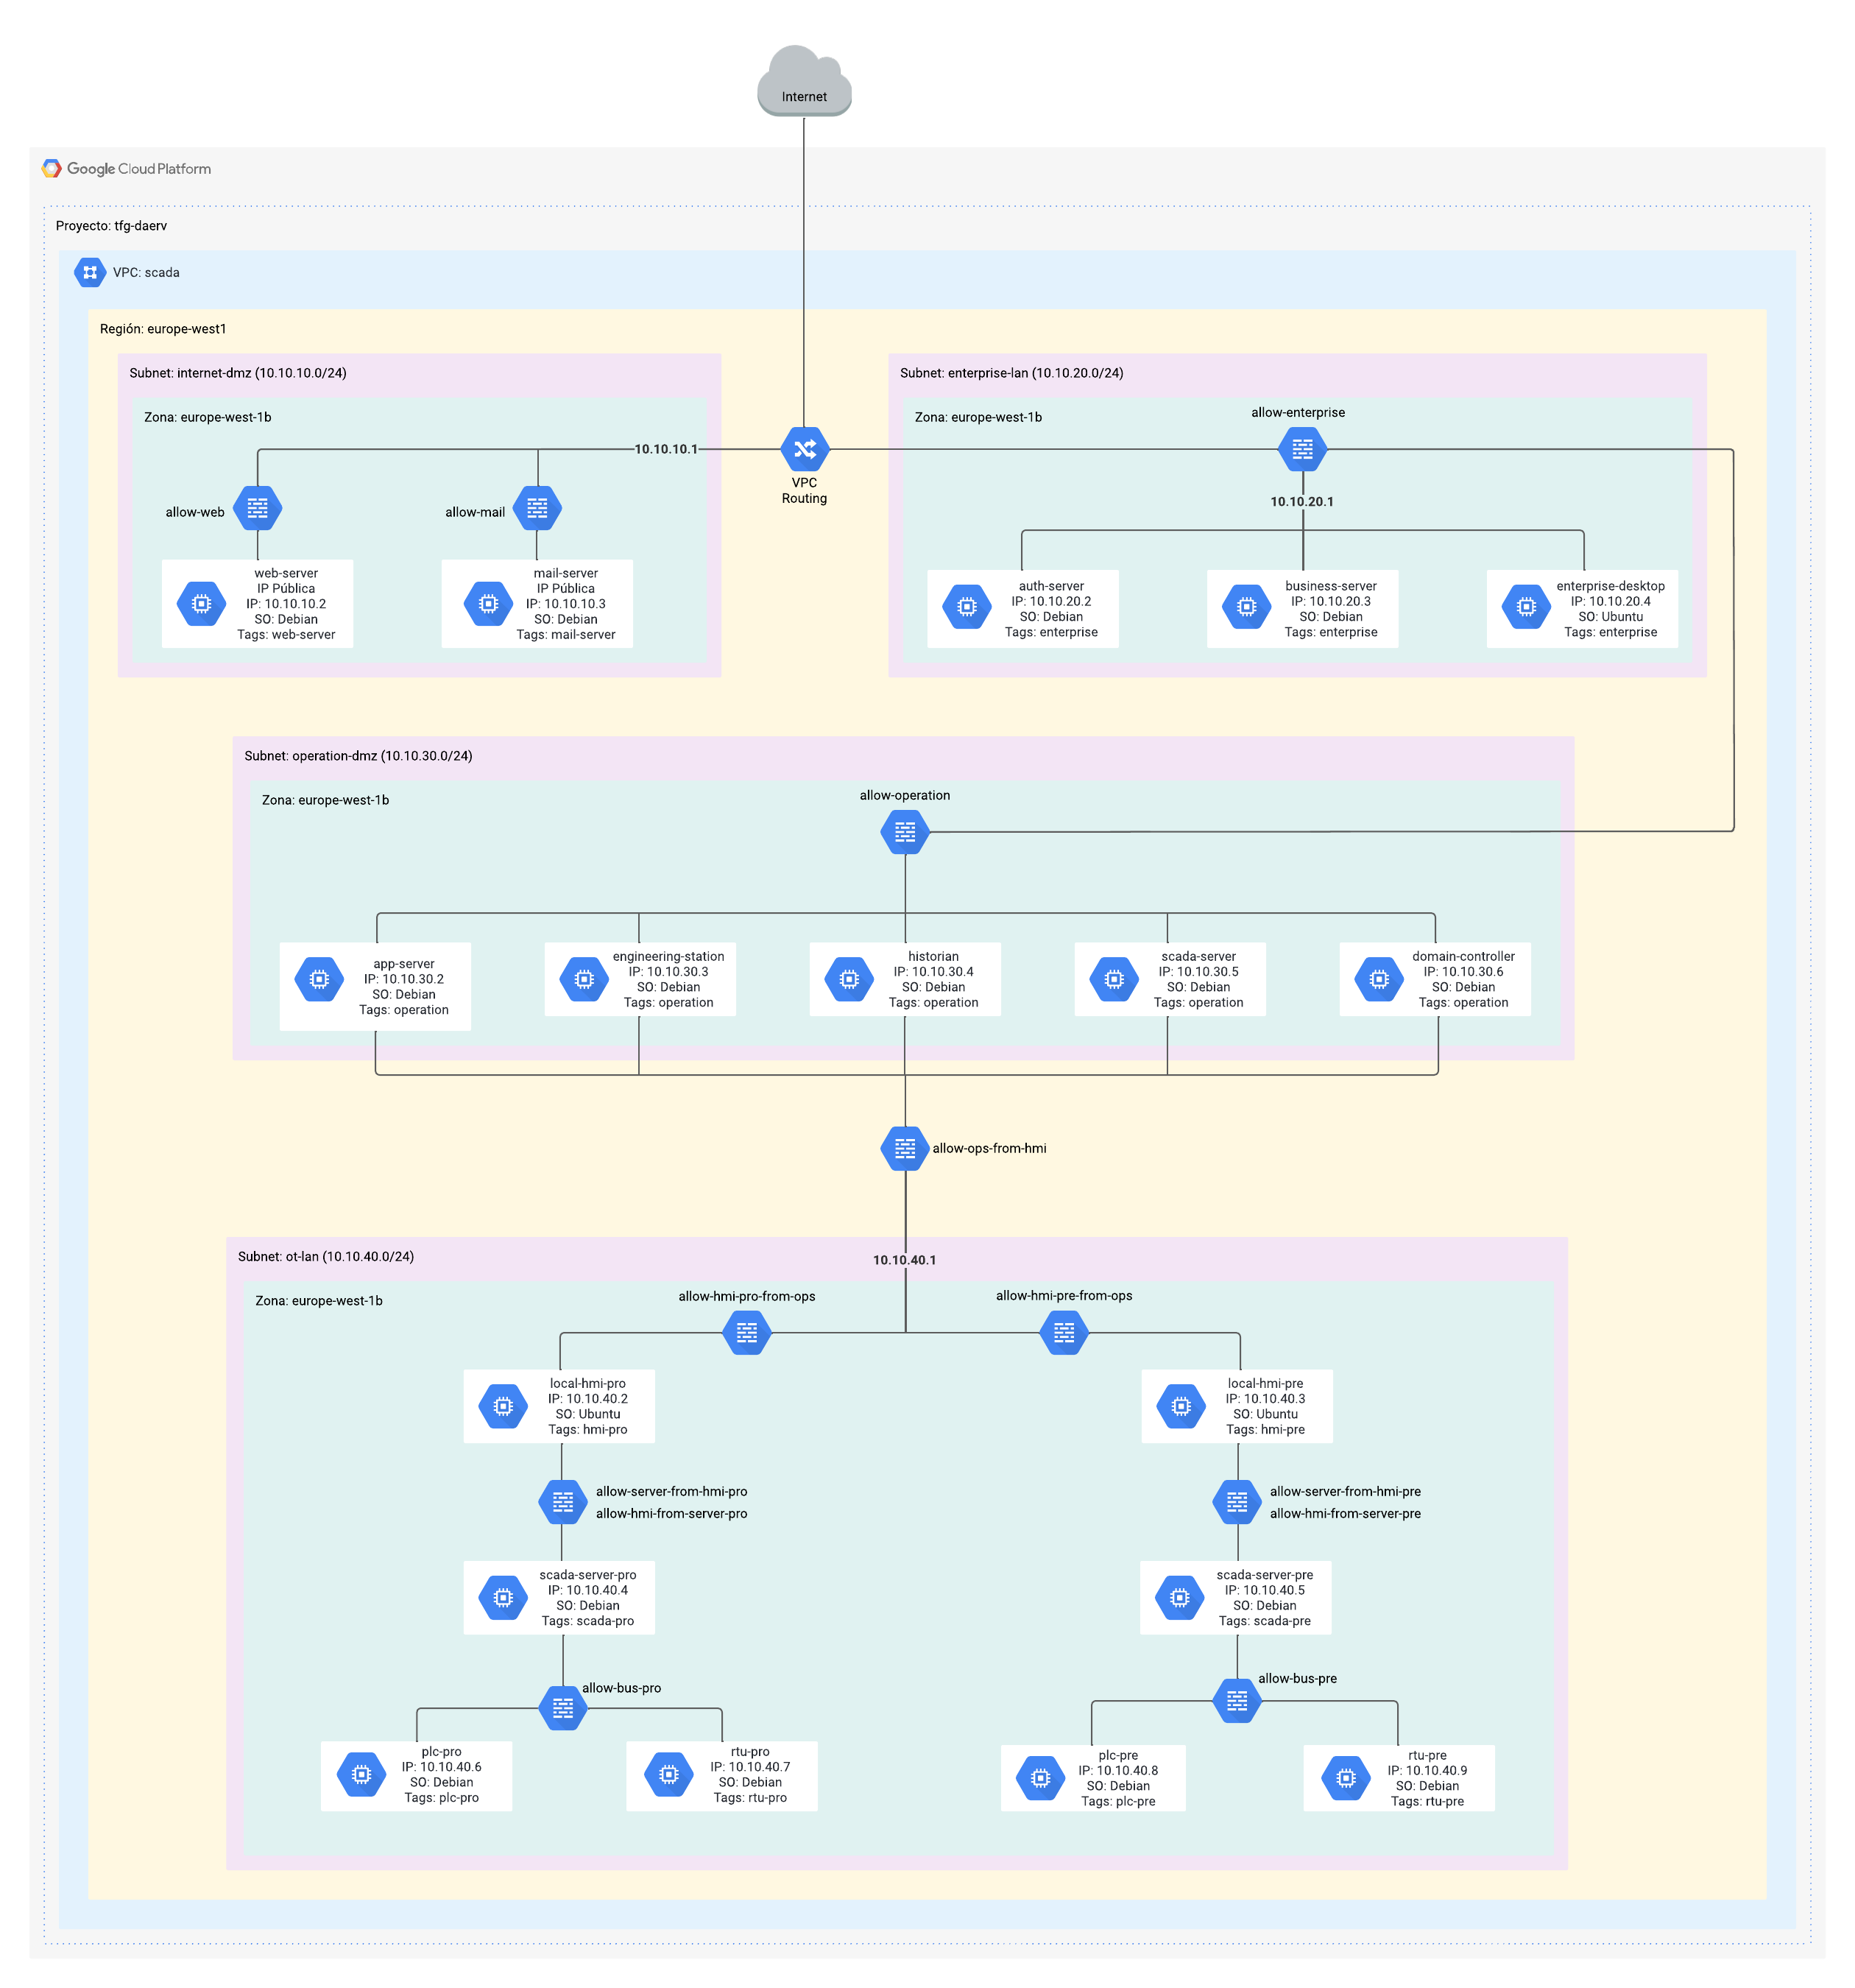
\includegraphics[width=\textwidth]{../imgs/desarrollo/escenarios-de-red/SCADA/EscenarioSCADA.png}
  \caption{Implementación en GCP del escenario SCADA}
  \label{fig:scada-i}
  \end{figure}
  \clearpage

    % Resultados
\chapter{Resultados y validación} \label{ch:res}
  Este capítulo presenta los resultados obtenidos tras el desarrollo del proyecto y su comprobación mediante pruebas. Para ello, para cada escenario se va a comprobar que la infraestructura se despliega correctamente y posteriormente se va a validar que la conectividad entre los equipos es la esperada.

\section{Escenarios Smart Office}
  Se va a validar el despliegue de los escenarios Smart Office. Dado que la implementación es muy similar en ambos, se va a mostrar las pruebas realizadas sobre uno de ellos.

\subsection{Despliegue de la infraestructura}
 Lo primero es navegar hasta el directorio en el que se encuentran los ficheros \texttt{.tf}. Una vez ahí, es necesario ejecutar la orden \texttt{terraform init} para que se configure el provider correctamente, seguida de la orden \texttt{terraform apply} para que Terraform elabore un plan para alcanzar el estado deseado. Tras ejecutar \texttt{terraform apply}, Terraform mostrará una lista de los recursos a crear, modificar o eliminar para cumplir con el estado que marcan los ficheros de configuración. Tras la lista, aparecerá un prompt en el que sólo si escribimos \texttt{yes} Terraform procede a ejecutar las acciones necesarias para el despliegue.

  \begin{figure}[h]
  \centering
  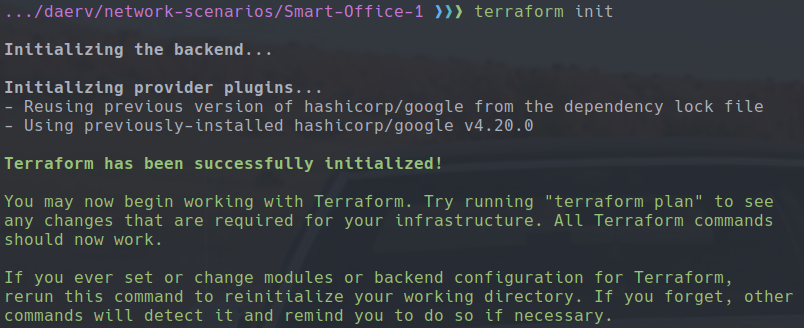
\includegraphics[width=0.8\textwidth]{../imgs/desarrollo/resultados/so/init.png}
  \caption{Ejecución del comando \texttt{terraform init}}
  \end{figure}
  
  \begin{figure}[h]
  \centering
  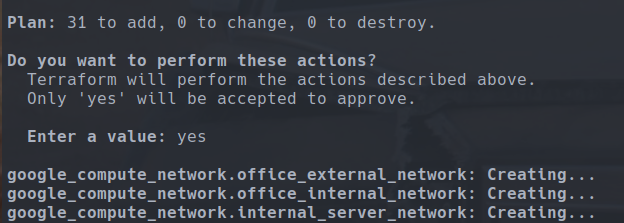
\includegraphics[width=0.8\textwidth]{../imgs/desarrollo/resultados/so/prompt.png}
  \caption{Prompt de confirmación tras la ejecución de \texttt{terraform apply}}
  \end{figure}

  Una vez se confirma la creación de los recursos, Terraform comienza a ejecutar el plan de creación de los recursos y va informando por la terminal sobre el estado de estos. Una vez se han creado todos, se nos informa y podemos ejecutar \texttt{terraform state list} para comprobar qué recursos hay desplegados: 

  \begin{figure}[h]
  \centering
  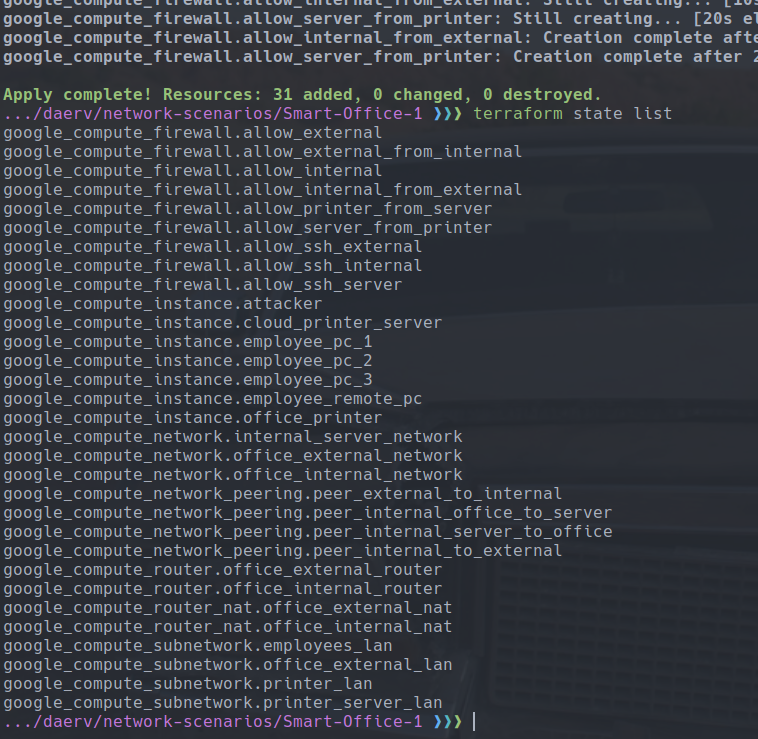
\includegraphics[width=0.75\textwidth]{../imgs/desarrollo/resultados/so/state.png}
  \caption{Ejecución del comando \texttt{terraform state list}}
  \end{figure}

  También podemos comprobar en GCP el despliegue de los diferentes elementos que componen el escenario accediendo a los distintos servicios, tal y como se muestra a continuación.

  \begin{figure}[h]
  \centering
  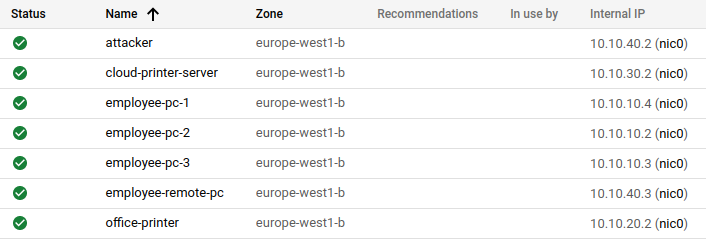
\includegraphics[width=\textwidth]{../imgs/desarrollo/resultados/so/instances.png}
  \caption{Instancias desplegadas en Google Compute Engine - Smart Office}
  \end{figure}

  \begin{figure}[h]
  \centering
  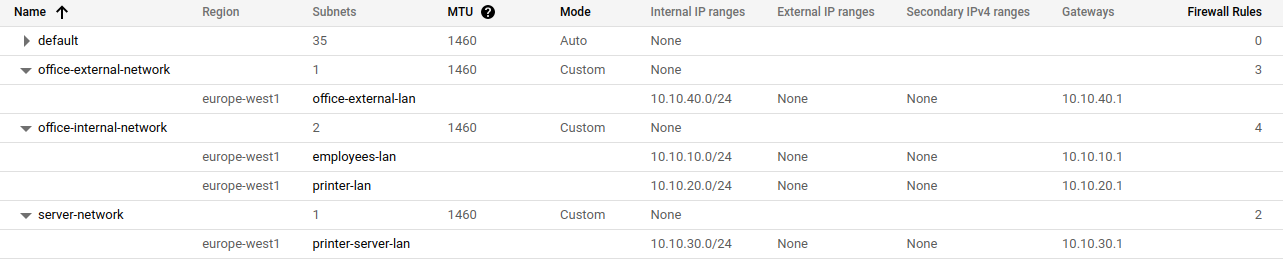
\includegraphics[width=\textwidth]{../imgs/desarrollo/resultados/so/vpcs.png}
  \caption{VPCs desplegadas - Smart Office}
  \end{figure}

  \begin{figure}[h]
  \centering
  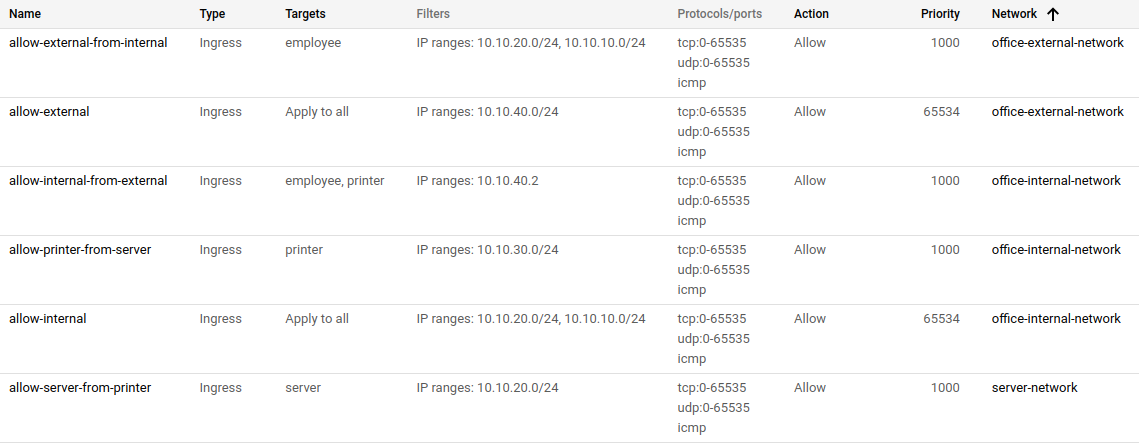
\includegraphics[width=\textwidth]{../imgs/desarrollo/resultados/so/fws.png}
  \caption{Reglas de FW aplicadas - Smart Office}
  \end{figure}
  \clearpage

\subsection{Tests}
  Para comprobar que la conectividad entre los elementos es la deseada según las reglas de firewall definidas en la tabla \ref{tab:fw1} se han creado una serie de tests de conectividad haciendo uso del servicio Network Intelligence de GCP:
  
  \begin{figure}[h]
  \centering
  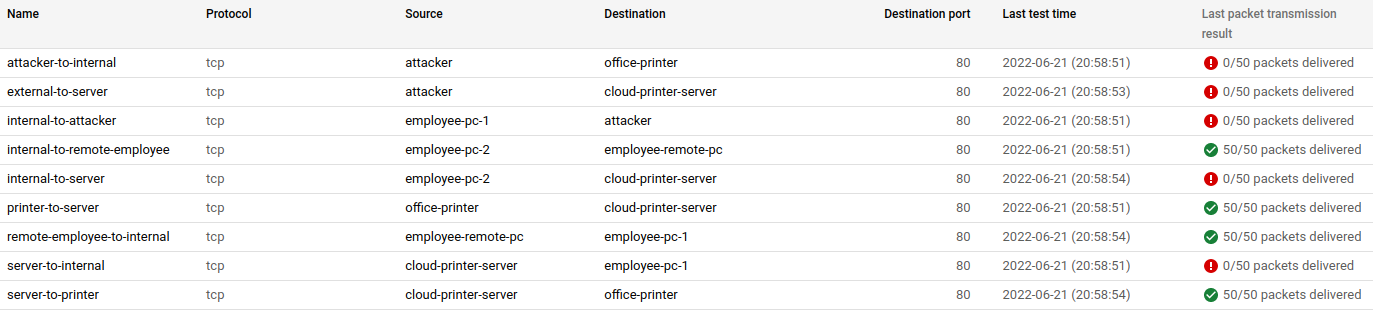
\includegraphics[width=\textwidth]{../imgs/desarrollo/resultados/so/tests.png}
  \caption{Tests de conectividad - Smart Office}
  \end{figure}

\section{Escenario Smart Home}
  Se van a presentar las mismas pruebas, esta vez para el escenario Smart Home. En este apartado, así como en el siguiente, se va a obviar la parte correspondiente a los comandos de Terraform para evitar redundancia. 

\subsection{Despliegue de la infraestructura}
  Se muestra a continuación como la infrestructura se ha creado correctamente en GCP:

  \begin{figure}[h]
  \centering
  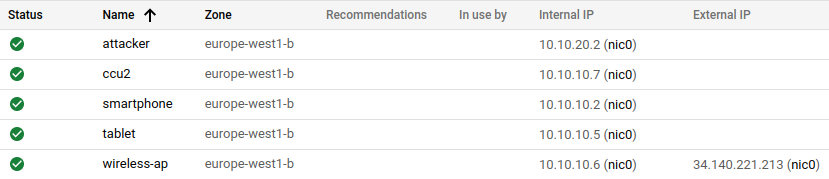
\includegraphics[width=\textwidth]{../imgs/desarrollo/resultados/sh/instances.png}
  \caption{Instancias desplegadas en Google Compute Engine - Smart Home}
  \end{figure}

  \begin{figure}[h]
  \centering
  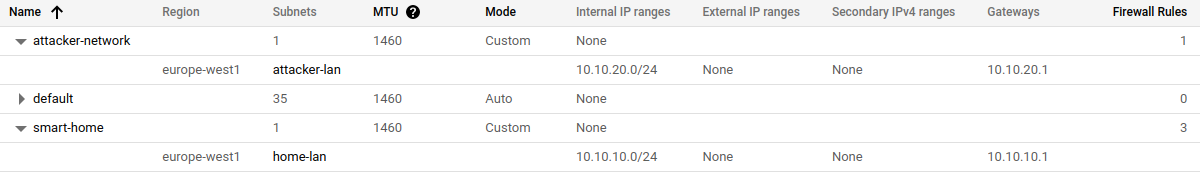
\includegraphics[width=\textwidth]{../imgs/desarrollo/resultados/sh/vpcs.png}
  \caption{VPCs desplegadas - Smart Home}
  \end{figure}
  \clearpage

  \begin{figure}[h]
  \centering
  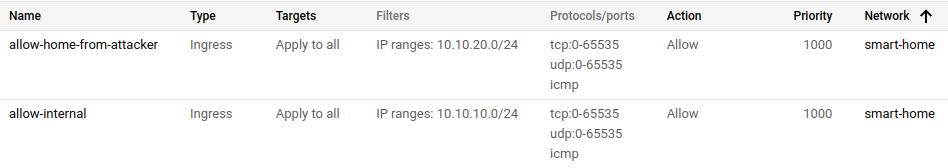
\includegraphics[width=\textwidth]{../imgs/desarrollo/resultados/sh/fws.png}
  \caption{Reglas de FW aplicadas - Smart Home}
  \end{figure}

\subsection{Tests}
  En este escenario se han definido los siguientes tests:

  \begin{figure}[h]
  \centering
  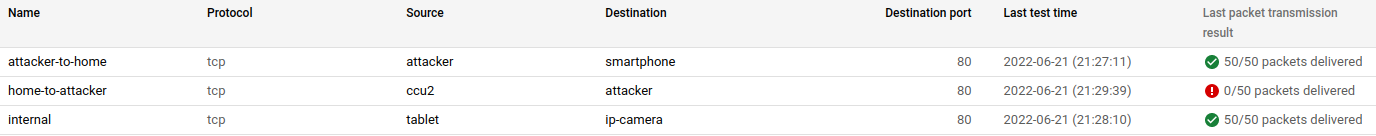
\includegraphics[width=\textwidth]{../imgs/desarrollo/resultados/sh/tests.png}
  \caption{Tests de conectividad - Smart Home}
  \end{figure}

  Adicionalmente, accedemos a una de las instancias de la red local de la casa a través de SSH (es necesario crear una regla de FW que lo permita) y vemos que tiene acceso a Internet a través de la IP pública de la instancia wireless-ap y que cuenta con Docker instalado, lo que verifica el funcionamiento de los scripts \texttt{proxy-config.tftpl} y \texttt{docker-proxy-provisioning.tftpl} pasados como parámetro:

  \begin{figure}[h]
  \centering
  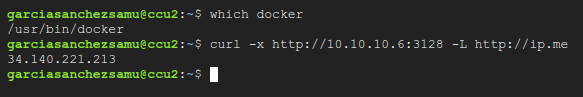
\includegraphics[width=\textwidth]{../imgs/desarrollo/resultados/sh/tests2.png}
  \caption{Tests de aprovisionamiento - Smart Home}
  \end{figure}
  \clearpage

\section{Escenario SCADA}
  Al igual que los apartados anteriores, se va a presentar el despliegue y los tests correspondientes al escenario SCADA.
  
\subsection{Despliegue de la infraestructura}
  A continuación se muestra, al igual que para el resto de escenarios, imágenes que verifican el despliegue de la infraestructura en Google Cloud. 

  \begin{figure}[h]
  \centering
  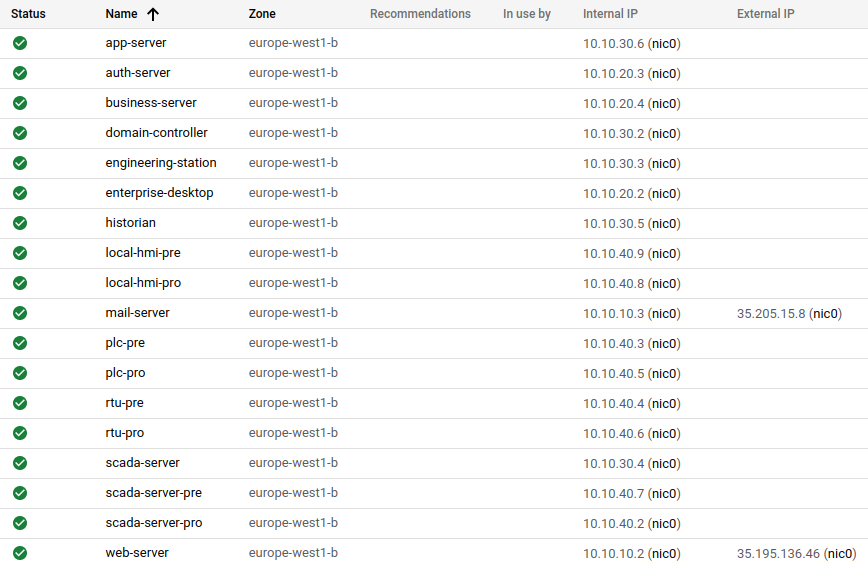
\includegraphics[width=\textwidth]{../imgs/desarrollo/resultados/scada/instances.png}
  \caption{Instancias desplegadas en Google Compute Engine - SCADA}
  \end{figure}

  \hfill{5cm}

  \begin{figure}[h]
  \centering
  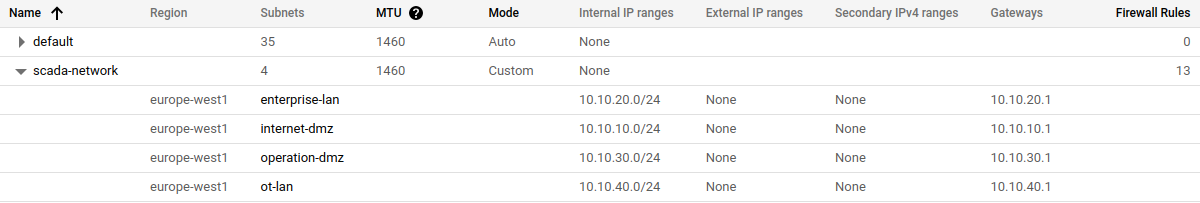
\includegraphics[width=\textwidth]{../imgs/desarrollo/resultados/scada/vpcs.png}
  \caption{VPCs desplegadas - SCADA}
  \end{figure}
  \clearpage

  \begin{figure}[t]
  \centering
  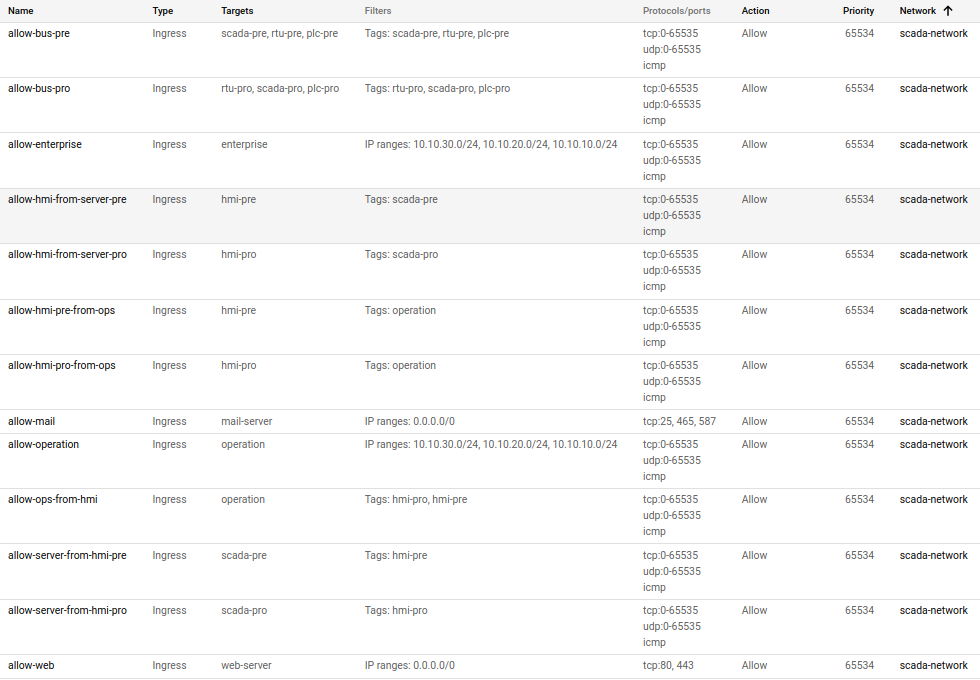
\includegraphics[width=\textwidth]{../imgs/desarrollo/resultados/scada/fws.png}
  \caption{Reglas de FW aplicadas - SCADA}
  \end{figure}
  
\subsection{Tests}
  Los siguientes tests de conectividad han sido definidos:

  \begin{figure}[h]
  \centering
  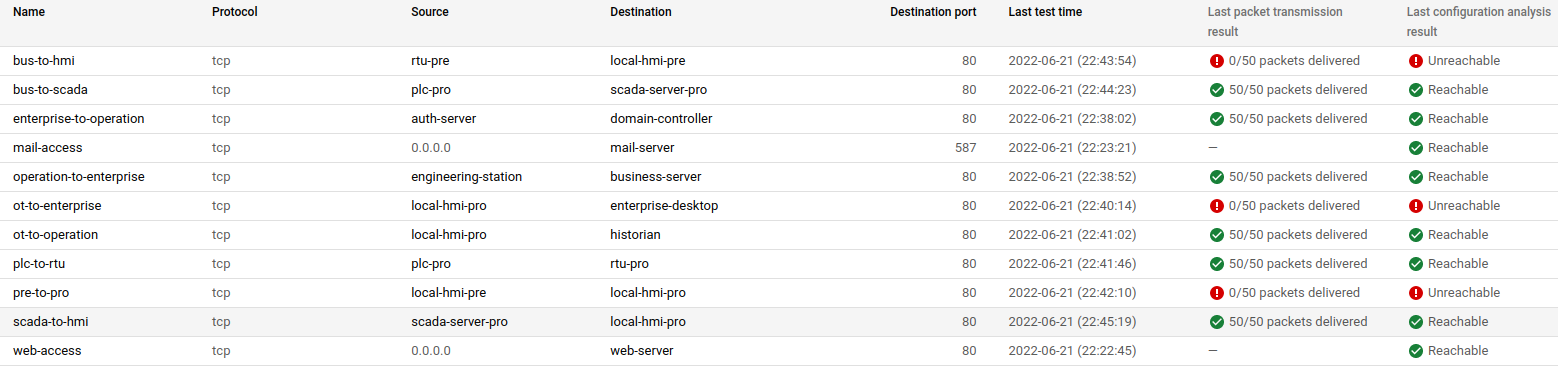
\includegraphics[width=\textwidth]{../imgs/desarrollo/resultados/scada/tests.png}
  \caption{Test de conectividad - SCADA}
  \end{figure}
  \clearpage

  Por último se verifica el funcionamiento del script \texttt{docker-provisioning.tftpl}. Para ello accedemos a la IP pública del servidor web desde el ordenador host y comprobamos que está ejecutando el software \textit{nginx} en el puerto 80.

  \begin{figure}[h]
  \centering
  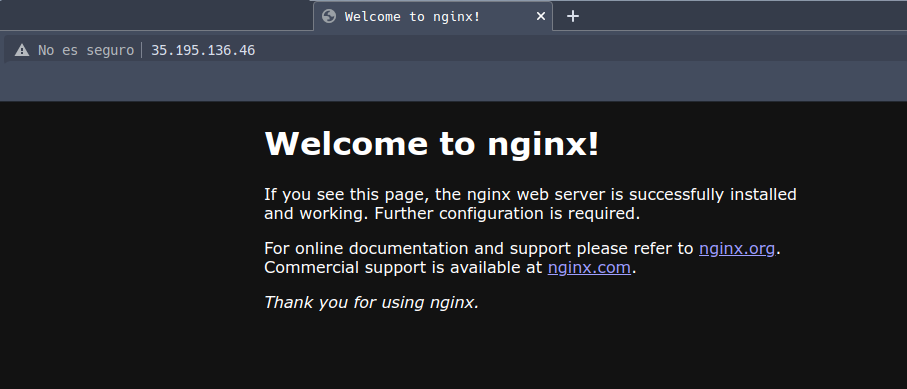
\includegraphics[width=\textwidth]{../imgs/desarrollo/resultados/scada/nginx.png}
  \caption{Test de aprovisionamiento - SCADA}
  \end{figure}

    % Conclusiones y llíneas futuras
\chapter{Conclusiones y líneas futuras} \label{ch:con}
  Este capítulo expone las conclusiones extraidas a raíz de la realización del proyecto y las líneas futuras en las que se puede seguir trabajando.

\section{Conclusiones} \label{sec:concs}
  En el último año se ha experimentado un más que notable aumento del número de ciberataques y sofisticación de las amenazas conocidas. Además, En la actualidad existe una gran demanda de perfiles de ciberseguridad. Este trabajo surge con la idea de hacer accesible y sencilla la práctica de ejerccicios de tipo Red Team para la formación en ejercicios de seguridad. El hecho de desplegar los escenarios en la nube con Terraform permite que cualquiera con permiso obtenga en cuestion de segundos un escenario funcional donde practicar y formarse, independientemente de donde se encuentre y el sistema que emplee.

\section{Líneas futuras} \label{sec:fut}
  Las líneas a seguir serían relacionadas con la configuración software de los elementos de los escenarios, de forma que se obtengan escenarios funcionales en los que practicar tests de intrusión específicos. Los ficheros que se proporcionan en el directorio \texttt{template-files} permiten aprovisionar las máquinas con imágenes Docker vulnerables, como las disponibles en el proyecto Vulhub. De esta forma, es posible crear servicios con vulnerabilidades conocidas de forma personalizada mediante un Dockerfile, alojarlas en DockerHub, y luego pasárselas como argumento a la instancia de Google Cloud a la hora de construirla, teniendo así un entorno funcional en el que practicar ejercicios de Red Team. De igual forma, para los sistemas operativos base (como Kali Linux en el caso del atacante) se pueden crear imágenes en Google Cloud a partir de la ISO correspondiente y desplegar la instancia usando esa imagen.

	%----------------------------------------------------------------------------------
	% Bibliografía
	\printbibliography[heading=bibintoc]
	\clearpage
	%----------------------------------------------------------------------------------
	% Anexos	
	% Anexos
\appendix
\clearpage
\addappheadtotoc
\appendixpage

\fancyhead[LO]{\small ANEXOS}
\fancyhead[RE]{\small ANEXOS}

\chapter{Aspectos éticos, económicos, sociales y ambientales } \label{anx:et}
  En este anexo se va a realizar una descripción de los aspectos éticos, económicos, sociales y ambientales surgidos de la realización del trabajo. 

\section*{Introducción}
  Este trabajo de fin de grado está integrado en el proyecto COBRA de la ETSIT, y su objetivo es optimizar la forma en la que se realiza actualmente el despliegue de los Cyber Range, en términos de velocidad, escalabilidad, portabilidad y seguridad. 

  Desde un punto de vista social, el principal colectivo afectado o asociado a la realización de este proyecto estaría estrechamente relacionado con el ámbito de la ETSIT. Considerando los planos económico, medioambiental y ético, el trabajo aporta valor en todos ellos, tal y como se va a detallar a continuación. 

\section*{Impactos relacionados con el proyecto}
  En primer lugar, el sistema desarrollado proporcionará una mayor productividad y calidad en la formación de los alumnos que cursen asignaturas de ciberseguridad así como programas de estudios relacionados con ella. Como ya se ha comentado en secciones anteriores, el despliegue en la nube supone un gran ahorro económico, ya que se paga únicamente por los recursos que se usan y durante el tiempo que se usan, de forma que en el caso de que no hubiera nadie practicando, no habría costes asociados. Además, es un entorno seguro, pues los escenarios son desplegados en una infraestructura completamente independiente del entorno de la organización, lo cual evita cualquier conflicto ético al no haber información o recursos sensibles de por medio\dots

  En cuanto al plano medioambiental, y estrechamente relacionado con el económico ya comentado, esta herramienta evita la compra innecesaria de dispositivos específicos para su empleo y uso. Esto se debe a que el sistema está completamente virtualizado, y por tanto es posible su despliegue completo en la nube, siendo por tanto compatible con cualquier tipo de ordenador, con independencia de su sistema operativo. Este aspecto permite reducir la huella ambiental al reducir los residuos a largo plazo.

  Adicionalmente, al estar el proyecto COBRA ligado al programa de gobierno COINCIDENTE, el sistema tendrá gran importancia de cara a la sociedad española, pues unos resultados positivos derivados del éxito del trabajo permitirían una mejor formación en los profesionales de ciberseguridad de España, lo que a su vez mejoraría la calidad de vida de las personas.

\section*{Análisis detallado de uno de los principales impactos}
  Tras la exposición en la sección anterior de los impactos más relevantes relacionados con el proyecto, podemos afirmar que uno de los más influyentes sería el plano económico-medioambiental asociado al despliegue en Cloud. 

  El hecho de poder virtualizar cualquier tipo de sistema proporciona una gran flexibilidad a la hora de definir escenarios completamente distintos entre sí y evita la compra de equipos específicamente para ello. Un Cyber Range que se despliega haciendo uso de equipos físicos corre el riesgo de que haya periodos de tiempo en los que no se use, lo cual no exime del pago de la infraestructura que se emplea. Mientras tanto, en la nube tanto el despliegue como el pago de la infraestructura es bajo demanda.

  Además, respecto al uso de GCP como proveedor cloud, cabe destacar que Google no tiene emisiones de carbono desde 2007 y se comprometió a operar con energía neutra de carbono en un 100\% las 24 horas, todos los días, para el año 2030. Los centros de datos de Google, incluidos los que ejecutan los servicios de Google Cloud, también usan mucho menos energía que los centros de datos típicos. Por este motivo, el uso de Google Cloud ayuda a reducir la huella de carbono de la infraestructura IT.

\section*{Conclusiones}
  A lo largo del desarrollo del proyecto se han realizado decisiones sobre requisitos y objetivos a cumplir que han sido claves para el alcance de un ecosistema que favorece al desarrollo sostenible y a la mejora de la sociedad. 

  Es por esto que podemos llegara a la conclusión de que todas las personas y organizaciones involucradas en el proyecto obtienen un beneficio e impacto positivo como consecuencia del uso del sistema desarrollado. 

\chapter{Presupuesto económico} \label{anx:ec}
  Este anexo presenta una estimación de los costes asociados a la realización de este trabajo de fin de grado y que han sido necesarios para la consecución de los objetivos. Se van a tener en cuenta para ello tanto los materiales utilizados como la mano de obra, a partir de los cuales se realizará una aproximación de los costes directos e indirectos. 

\section*{Costes de mano de obra}
  Para estimar el coste asociado a la mano de obra, en primer lugar se ha realizado una aproximación del número de horas empleadas en las diferentes etapas de realización del proyecto. Esta aproximación se muestra con detalle en la tabla inferior. 
  
  \begin{table}[h]
    \begin{center}
      \begin{tabular}{ | m{13,5cm} | w{c}{1,5cm} | }
        \hline\rowcolor{oranget} \centering\textbf{Subproceso} & \textbf{Horas} \\ \hline
        Estudio de las diferentes tecnologías (Terraform, Google Cloud) & 90 \\ \hline\rowcolor{oranger}
        Análisis de los escenarios (vector de ataque y conexiones necesarias entre los elementos) & 40 \\ \hline
        Diseño e implementación de los escenarios en Google Cloud & 130 \\ \hline\rowcolor{oranger}
        Desarrollo de herramientas de configuración & 30  \\ \hline\
        Pruebas & 40  \\ \hline\rowcolor{oranger}
        Elaboración de la memoria & 75 \\ \hline\rowcolor{total}
        \textbf{Total} & \textbf{405} \\ \hline
      \end{tabular}
      \caption{Horas asociadas a cada una de los subprocesos de realización del proyecto}
      \label{tab:hours}
    \end{center}
  \end{table}
  
  Una vez obtenida una aproximación de las horas empleadas en todo el proceso de diseño y desarollo del sistema, se va a considerar el salario medio anual de un Ingeniero de Telecomunicación junior para estimar el coste de mano de obra. Según el informe llevado a cabo por el Colegio Oficial de Ingenieros de Telecomunicación (COIT) en su Mapa socio-profesional del titulado en Ingeniería de Telecomunicación~\cite{anx1}, el salario medio anual de los titulados entre 18 y 24 años es de 23.553€, que con un contrato de 40h semanales y estimando 48 semanas laborales anuales resultaría en 12.27€/hora. Con este dato podemos finalmente estimar el coste de la mano de obra:

  \begin{table}[h]
    \begin{center}
      \begin{tabular}{ | c | c | c | }
        \hline \hline
        \multicolumn{3}{c}{Costes de mano de obra} \\ \hline \hline
        \hline \centering\textbf{Horas}\cellcolor{oranget} & \textbf{€/Hora}\cellcolor{oranget} & \textbf{Total}\cellcolor{total} \\ \hline
        405 & 12.27 & \textbf{4.969,35€}\cellcolor{total} \\ \hline
      \end{tabular}
      \caption{Costes de mano de obra}
      \label{tab:man}
    \end{center}
  \end{table}

\section*{Costes materiales}
  Para los costes materiales se tendrá en cuenta el ordenador personal con el que se ha realizado todo el desarrollo. Dicho equipo es un HP Pavilion 15-cs0012ns, que cuenta con un procesador Intel Core i7, una pantalla de 15.6" y 16GB de memoria RAM como algunas de sus características principales. Este ordenador tiene un coste aproximado de 1.100€. Además, se ha calculado la amortización mensual en base a los 4 años de antigüedad que tiene y esta se ha multiplicado por el número de meses en los que se ha estado trabajando en el proyecto (Octubre-Junio) para obtener la amortización total.

  También se ha de tener en cuenta que para la simulación de los escenarios fue necesario el uso de servicios de GCP que quedan fuera de la capa gratuita que ofrece Google y que por tanto tienen un coste asociado al tiempo que se han usado durante el desarrollo y las pruebas. En la imagen inferior se adjunta un reporte de los gastos en dichos servicios a lo largo del tiempo, acompañados del montante total. 

  \begin{figure}[h]
  \centering
  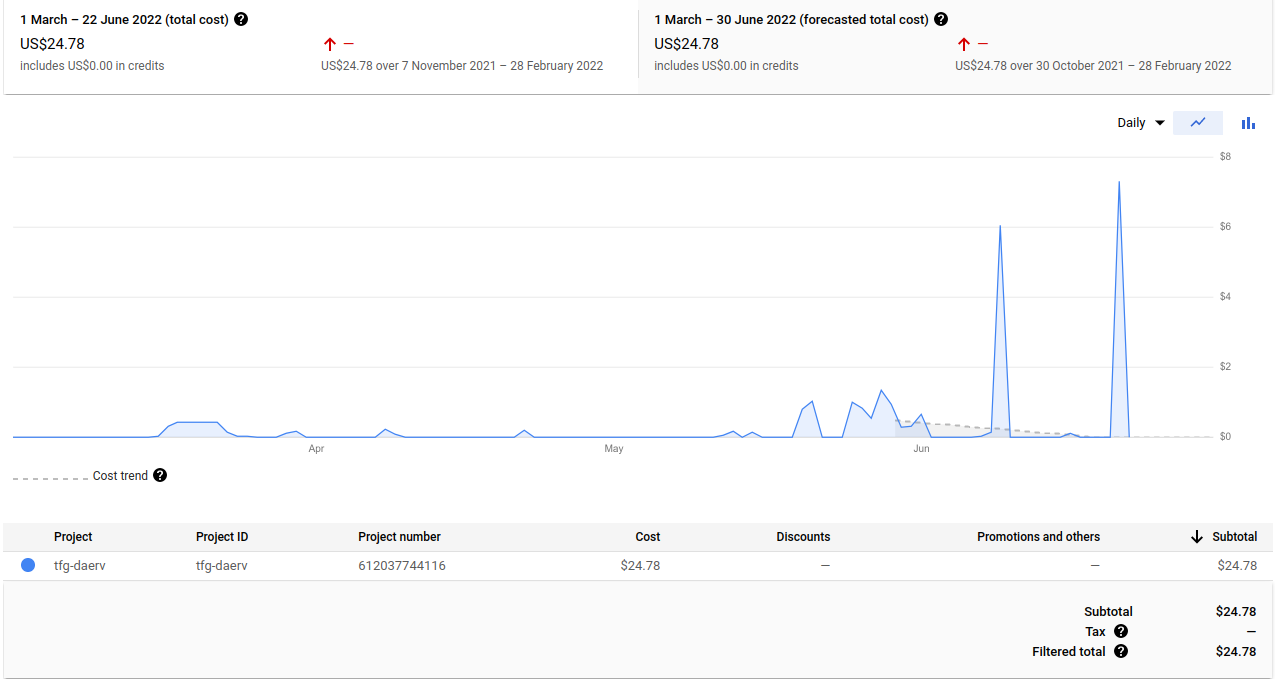
\includegraphics[width=\textwidth]{../imgs/desarrollo/facturacion/graph.png}
  \caption{Resumen de pagos en servicios de GCP}
  \end{figure}

  Como se puede apreciar, el gasto total ha sido de 24.78\$, que con la equivalencia actual (1€=1.06USD) serían 23,41€. Este dato nos permite cerrar los costes materiales como se puede ver a continuación.

  \clearpage
  \begin{table}[t]
    \begin{center}
      \begin{tabular}{ | c | m{2,5cm} | c | m{2,75cm} | m{1,75cm} | c | }
        \hline \hline
        \multicolumn{6}{c}{Costes materiales} \\ \hline \hline
        \hline \centering\textbf{Material}\cellcolor{oranget} & \textbf{Tiempo de vida (años)}\cellcolor{oranget} & \textbf{Precio}\cellcolor{oranget} & \centering\textbf{Amortización (€/mes)}\cellcolor{oranget} & \centering\textbf{Uso (meses)}\cellcolor{oranget} & \textbf{Total}\cellcolor{oranget} \\ \hline
        Ordenador portátil & \centering4 & 1.100€ & \centering22.92 & \centering8 & \textbf{183,36€} \\ \hline\rowcolor{oranger}
        Servicios GCP & \centering- & 23,41€ & \centering- & \centering- & \textbf{23,41€} \\ \hline\rowcolor{total}
        \multicolumn{5}{|c|}{\textbf{Total}} & \textbf{206,77€} \\ \hline
      \end{tabular}
      \caption{Costes materiales}
      \label{tab:mat}
    \end{center}
  \end{table}
    
\section*{Costes indirectos}
  Se han estimado los costes indirectos (como pueden ser luz, agua o internet) en un 20\% sobre la suma de los costes de mano de obra y material:
  
  \begin{table}[h]
    \begin{center}
      \begin{tabular}{ | c | c | c | }
        \hline \hline
        \multicolumn{3}{c}{Costes indirectos} \\ \hline \hline
        \hline \centering\textbf{Coste directo}\cellcolor{oranget} & \textbf{Estimación}\cellcolor{oranget} & \textbf{Total}\cellcolor{total} \\ \hline
         5.176,12€ & 20\% & \textbf{1.035,224€}\cellcolor{total} \\ \hline
      \end{tabular}
      \caption{Costes indirectos}
      \label{tab:ind}
    \end{center}
  \end{table}

\section*{Costes totales}
  Para terminar, se incluyen el IVA y el beneficio industrial para obtener los costes totales asociados al proyecto:

  \begin{table}[h]
    \begin{center}
      \begin{tabular}{ | c | c | c | }
        \hline \hline
        \multicolumn{3}{c}{Costes totales} \\ \hline \hline
        \hline \multicolumn{2}{|c|}{\textbf{Concepto}\cellcolor{oranget}} & \textbf{Coste}\cellcolor{oranget} \\ \hline
        \multirow{3}{*}{Costes directos} & Mano de obra & 4.969,35€ \\ \cline{2-3} 
         & Material & 206,77€ \\ \cline{2-3} 
         & \textbf{Total} & \textbf{5.176,12€} \\ \hline\rowcolor{oranger}
        \multicolumn{2}{|c|}{Costes indirectos} & 1.035,22€ \\ \hline
        \multicolumn{2}{|c|}{Total antes de beneficios e impuestos} & 6.211,34€ \\ \hline\rowcolor{oranger}
        \multicolumn{2}{|c|}{Beneficio industrial (10\%)} & 621,13€ \\ \hline
        \multicolumn{2}{|c|}{Total antes de impuestos} & 6.832,48€ \\ \hline\rowcolor{oranger}
        \multicolumn{2}{|c|}{IVA (21\%)} & 1.434,82€ \\ \hline\rowcolor{total}
        \multicolumn{2}{|c|}{\textbf{Total}} & \textbf{8.267,30€} \\ \hline
      \end{tabular}
      \caption{Costes totales}
      \label{tab:tot}
    \end{center}
  \end{table}

\chapter{Ficheros de configuración del escenario Smart Office 1} \label{anx:soI}
  Este anexo incluye todos los ficheros empleados para la configuración de la infrestructura del escenario Smart Office 1. El fichero main.tf contiene configuraciones generales, como son la configuración del provider de google, los peerings/VPN entre las VPC, o las reglas de firewall que controlan el tráfico que se intercambia entre las instancias. Adicionalmente, a fin de simplificar la lectura del código, hay un fichero .tf por cada una de las VPC, que contiene el código correspondiente a los elementos de red que la componen. Finalmente, en los ficheros variables.tf y terraform.tfvars se encuentran definidas las variables que se emplean en el resto del código.

\section*{main.tf} 
\lstinputlisting[language=Bash]{../../daerv/network-scenarios/Smart-Office-1/main.tf}

\section*{office-internal-network.tf}
\lstinputlisting[language=Bash]{../../daerv/network-scenarios/Smart-Office-1/office-internal-network.tf}
\clearpage

\section*{office-external-network.tf}
\lstinputlisting[language=Bash]{../../daerv/network-scenarios/Smart-Office-1/office-external-network.tf}

\section*{internal-server-network.tf}
\lstinputlisting[language=Bash]{../../daerv/network-scenarios/Smart-Office-1/internal-server-network.tf}
\clearpage

\section*{variables.tf}
\lstinputlisting[language=Bash]{../../daerv/network-scenarios/Smart-Office-1/variables.tf}

\chapter{Ficheros de configuración del escenario Smart Office 2} \label{anx:soII}
  Este anexo incluye todos los ficheros empleados para la configuración de la infrestructura del escenario Smart Office 2. El fichero main.tf contiene configuraciones generales, como son la configuración del provider de google, los peerings/VPN entre las VPC, o las reglas de firewall que controlan el tráfico que se intercambia entre las instancias. Adicionalmente, a fin de simplificar la lectura del código, hay un fichero .tf por cada una de las VPC, que contiene el código correspondiente a los elementos de red que la componen. Finalmente, en los ficheros variables.tf y terraform.tfvars se encuentran definidas las variables que se emplean en el resto del código.

\section*{main.tf} 
\lstinputlisting[language=Bash]{../../daerv/network-scenarios/Smart-Office-2/main.tf}

\section*{office-internal-network.tf}
\lstinputlisting[language=Bash]{../../daerv/network-scenarios/Smart-Office-2/office-internal-network.tf}

\section*{office-external-network.tf}
\lstinputlisting[language=Bash]{../../daerv/network-scenarios/Smart-Office-2/office-external-network.tf}

\section*{internal-server-network.tf}
\lstinputlisting[language=Bash]{../../daerv/network-scenarios/Smart-Office-2/internal-server-network.tf}

\section*{variables.tf}
\lstinputlisting[language=Bash]{../../daerv/network-scenarios/Smart-Office-2/variables.tf}

\chapter{Ficheros de configuración del escenario Smart Home} \label{anx:sh}
  Este anexo incluye todos los ficheros empleados para la configuración de la infrestructura del escenario Smart Home. El fichero main.tf contiene configuraciones generales, como son la configuración del provider de google, los peerings/VPN entre las VPC, o las reglas de firewall que controlan el tráfico que se intercambia entre las instancias. Adicionalmente, a fin de simplificar la lectura del código, hay un fichero .tf por cada una de las VPC, que contiene el código correspondiente a los elementos de red que la componen. Finalmente, en los ficheros variables.tf y terraform.tfvars se encuentran definidas las variables que se emplean en el resto del código.

\section*{main.tf} 
\lstinputlisting[language=Bash]{../../daerv/network-scenarios/Smart-Home/main.tf}

\section*{home-network.tf}
\lstinputlisting[language=Bash]{../../daerv/network-scenarios/Smart-Home/home-network.tf}

\section*{attacker-network.tf}
\lstinputlisting[language=Bash]{../../daerv/network-scenarios/Smart-Home/attacker-network.tf}

\section*{variables.tf}
\lstinputlisting[language=Bash]{../../daerv/network-scenarios/Smart-Home/variables.tf}

\chapter{Ficheros de configuración del escenario SCADA} \label{anx:scada}
  Este anexo incluye todos los ficheros empleados para la configuración de la infrestructura del escenario SCADA. El fichero main.tf contiene configuraciones generales, como son la configuración del provider de google, los peerings/VPN entre las VPC, o las reglas de firewall que controlan el tráfico que se intercambia entre las instancias. Adicionalmente, a fin de simplificar la lectura del código, hay un fichero .tf por cada una de las VPC, que contiene el código correspondiente a los elementos de red que la componen. Finalmente, en los ficheros variables.tf y terraform.tfvars se encuentran definidas las variables que se emplean en el resto del código.

\section*{main.tf} 
\lstinputlisting[language=Bash]{../../daerv/network-scenarios/SCADA/main.tf}

\section*{scada-network.tf}
\lstinputlisting[language=Bash]{../../daerv/network-scenarios/SCADA/scada-network.tf}

\section*{variables.tf}
\lstinputlisting[language=Bash]{../../daerv/network-scenarios/SCADA/variables.tf}

\chapter{Ficheros de aprovisionamiento} \label{anx:aprov}
  Este anexo incluye todos los ficheros empleados para la configuración y aprovisionamiento de las instancias de Compute Engine. El fichero docker-provisioning.tftpl permite instalar Docker en las máquinas Linux en función del sistema operativo, y posteriormente arrancar un contenedor especificando los parámetros 'argumentos', 'imagen' y 'tag'. El fichero proxy-config.tftpl permite configurar una instancia como proxy de acceso a internet, de forma que las instancias que no tengan conexión a internet pueden ser aprovisionadas accediendo a través de ella, haciendo uso del fichero docker-proxy-provisioning.tftpl.

\section*{docker-provisioning.tftpl} 
\lstinputlisting[language=Bash]{../../daerv/provisioning-files/docker-provisioning.tftpl}
\clearpage

\section*{docker-proxy-provisioning.tftpl} 
\lstinputlisting[language=Bash]{../../daerv/provisioning-files/docker-proxy-provisioning.tftpl}

\section*{proxy-config.tftpl} 
\lstinputlisting[language=Bash]{../../daerv/provisioning-files/proxy-config.tftpl}

	%----------------------------------------------------------------------------------
\end{document}
